  % High vs low arrest states pretrends

  \begin{figure}[h]
    \centering
    \caption{College Enrollment By States with High vs Low Black Adult Drug Arrest Rates}%
    \subfloat[\centering 1986]{{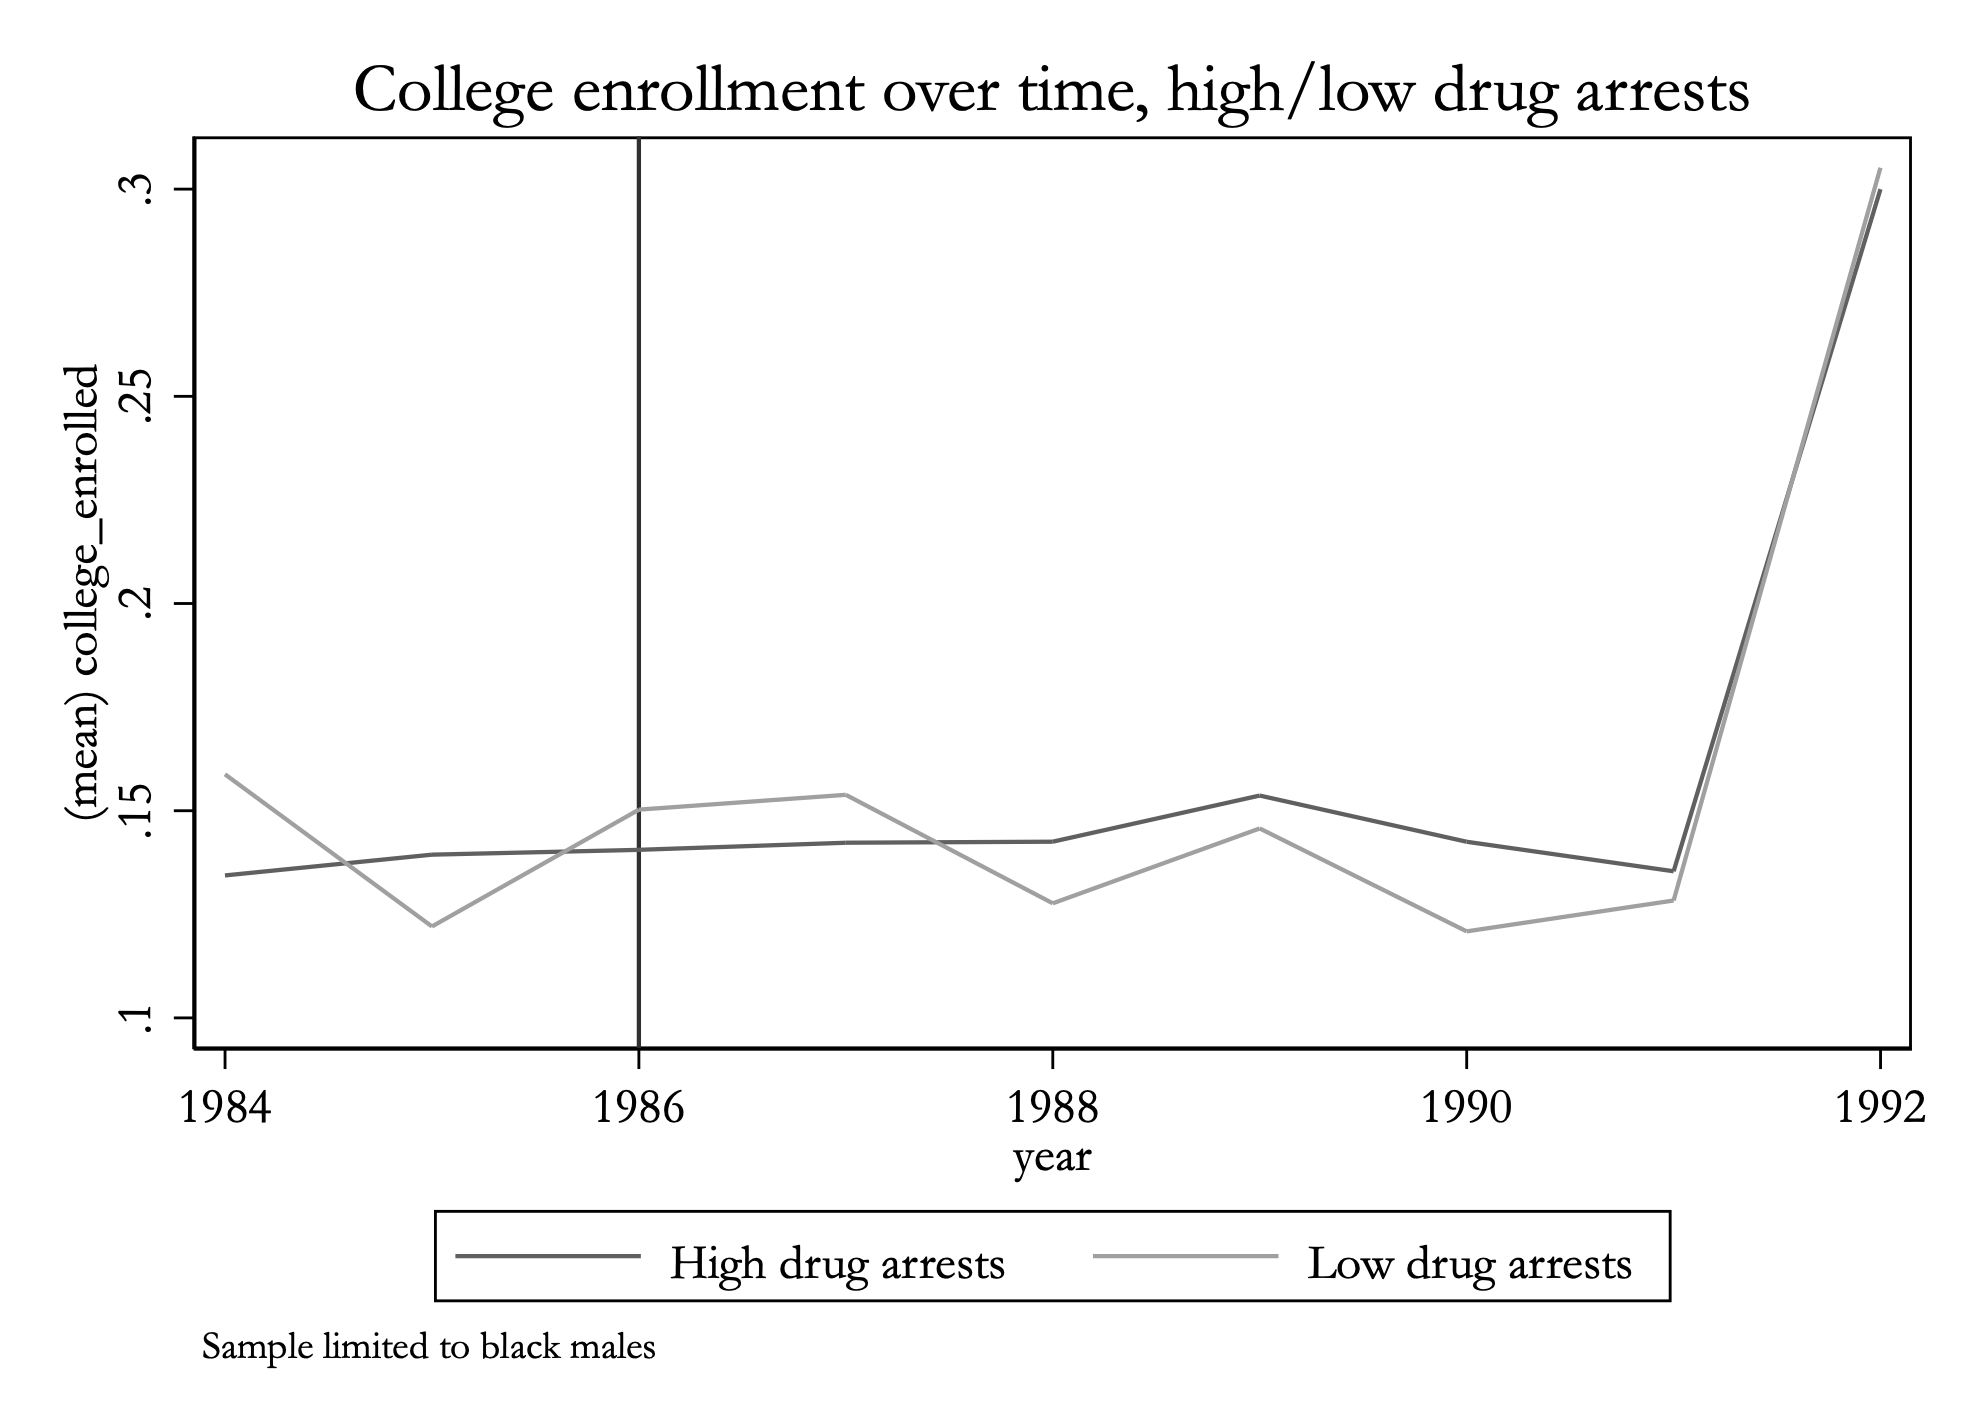
\includegraphics[width=7cm]{pretrends/1986/college_enroll_bydrugarrests_1986.png} }}%
    \qquad
    \subfloat[\centering 2010]{{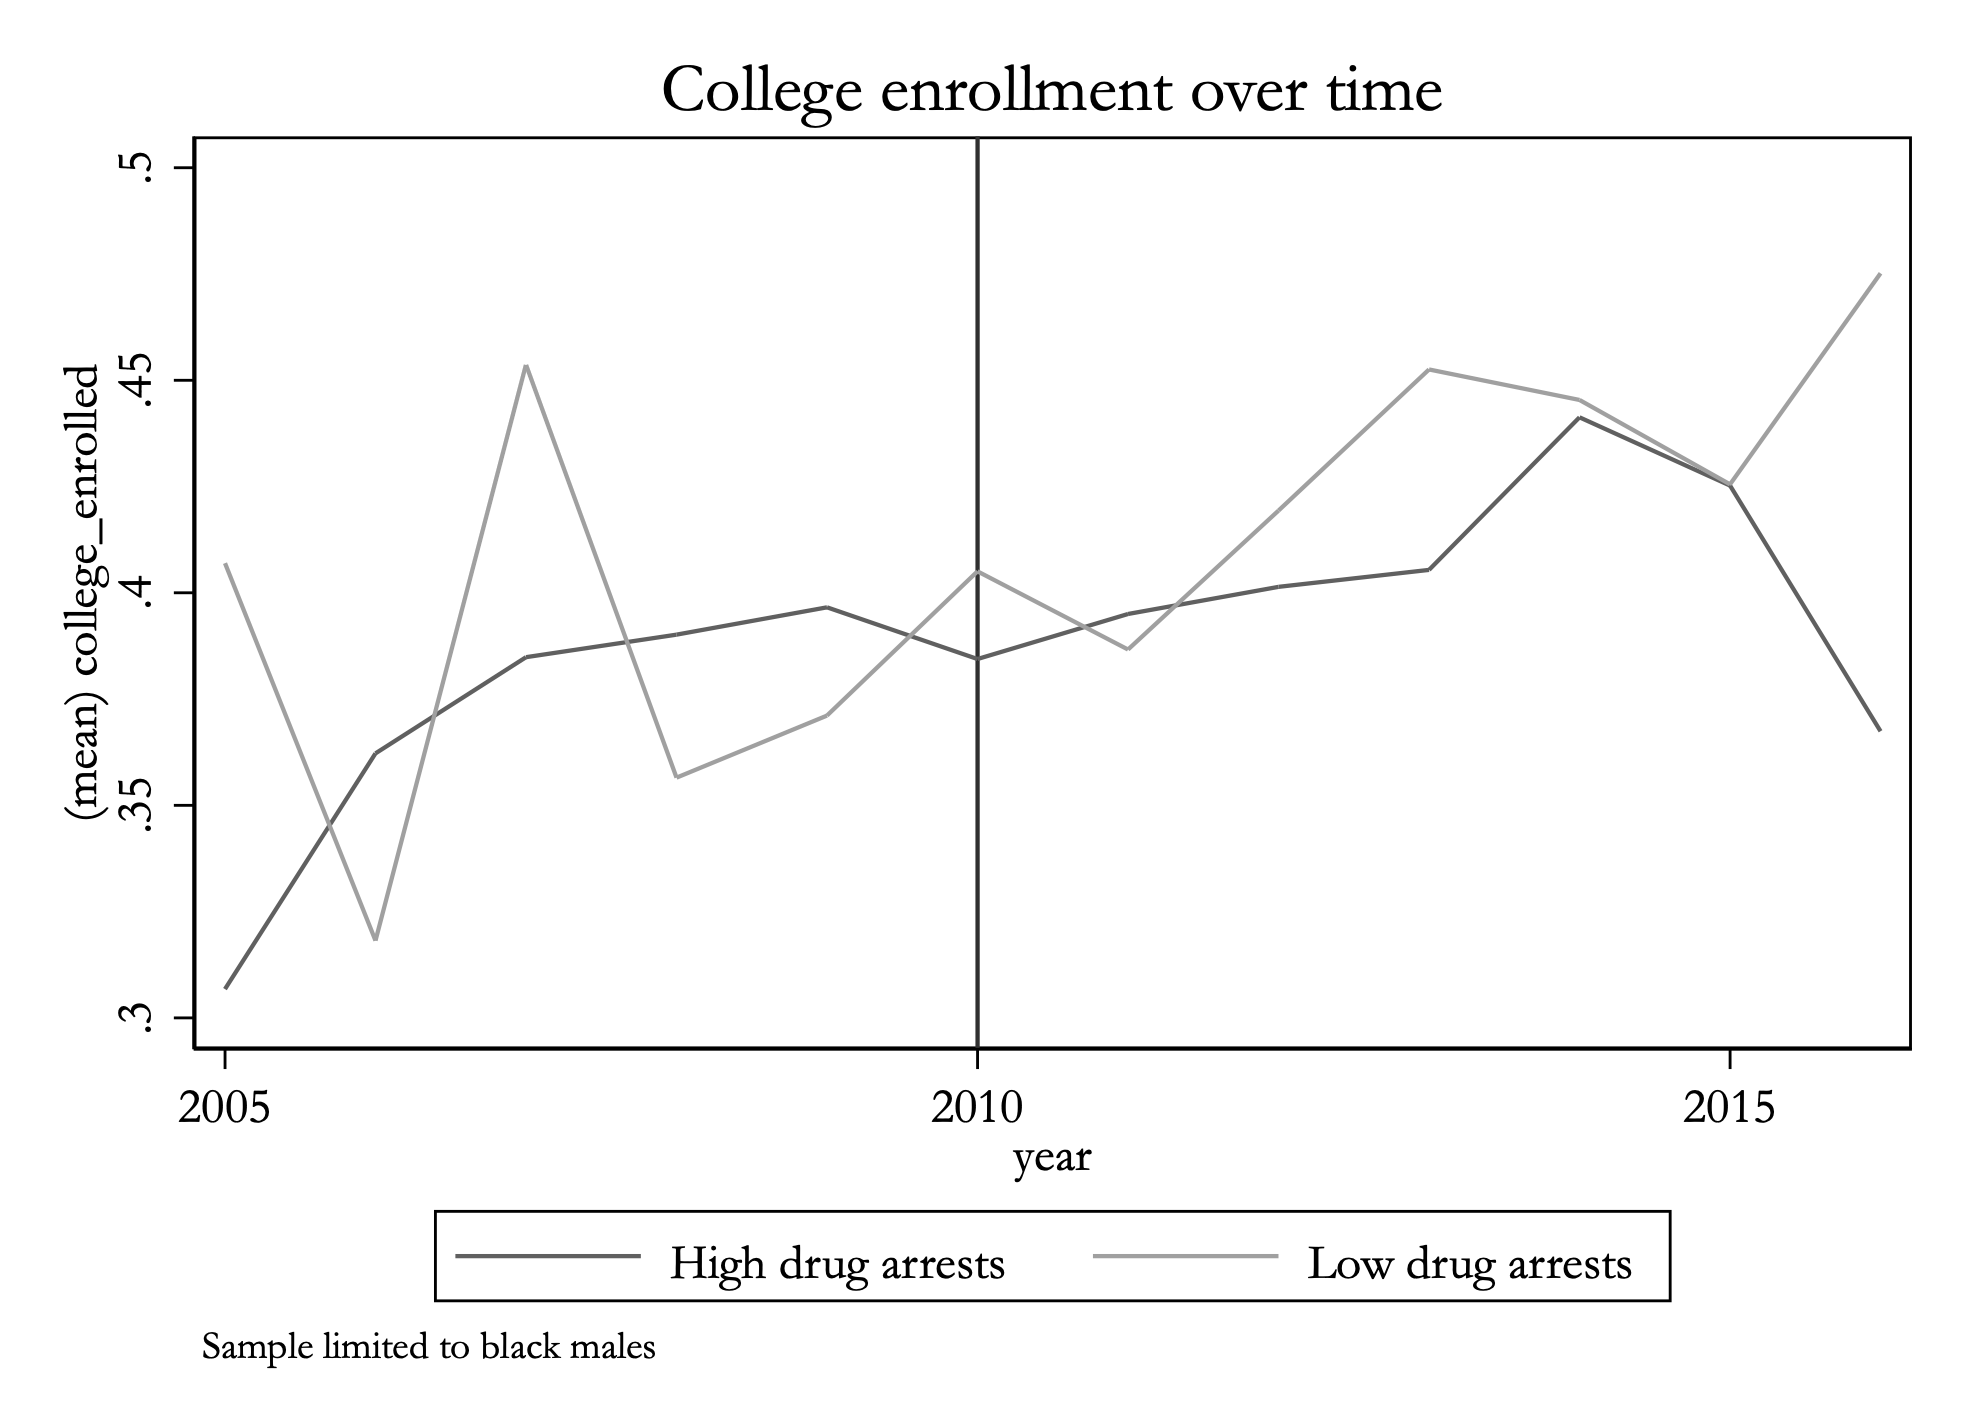
\includegraphics[width=7cm]{pretrends/2010/college_enroll_bydrugarrests_2010.png} }}%
    \label{fig:raw_college_highlowab_1986}%
  \end{figure}
  \begin{figure}[h]
    \centering
    \caption{College Enrollment By States with High vs Low Black Juvenile Drug Arrest Rates}%
    \subfloat[\centering 1986]{{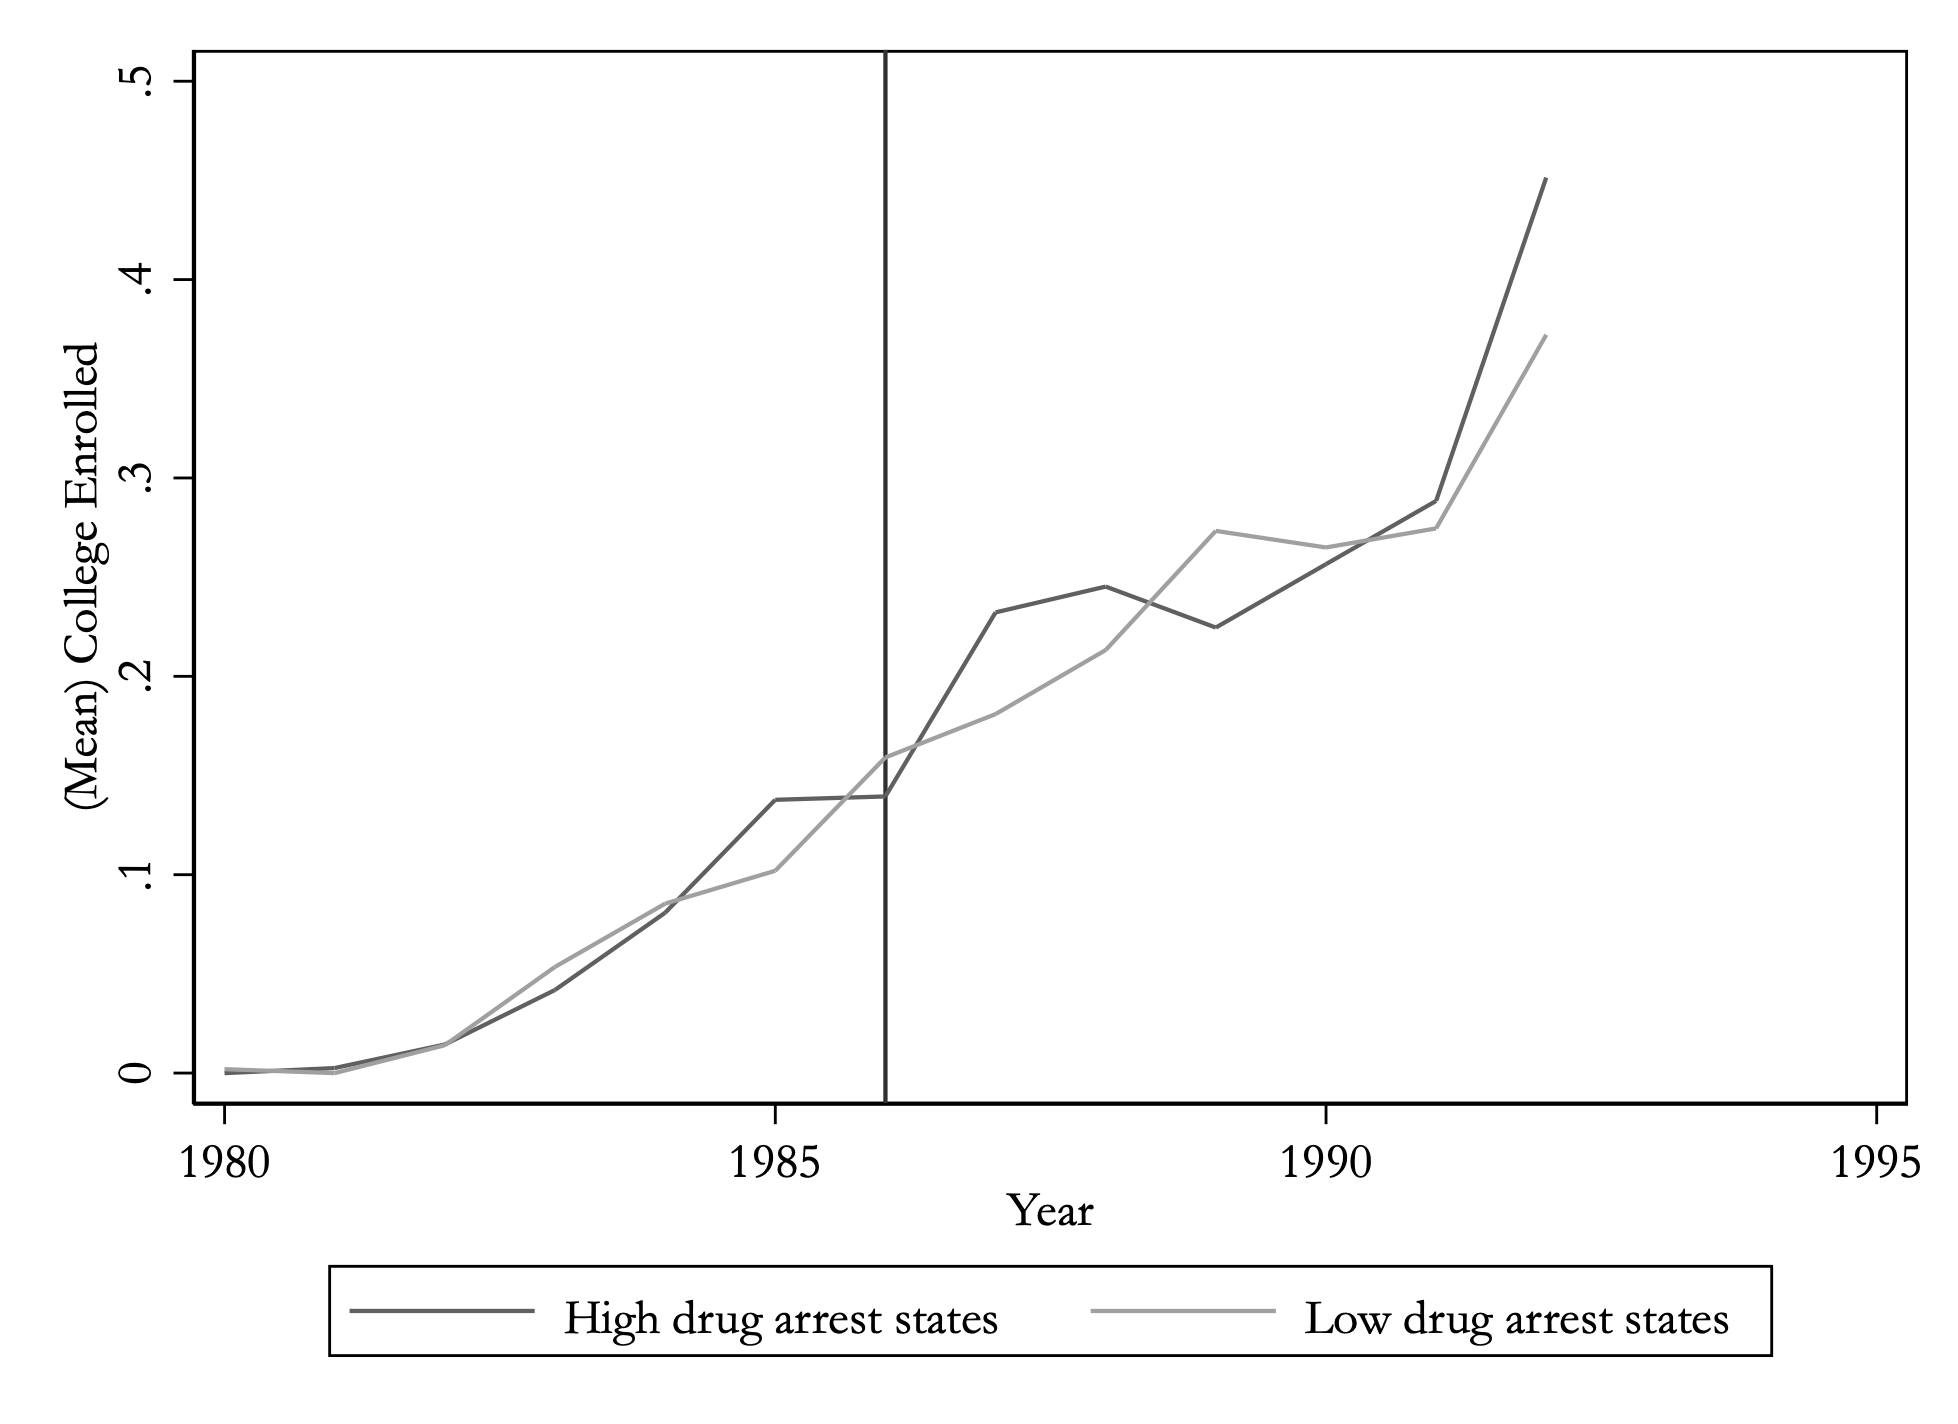
\includegraphics[width=7cm]{pretrends/1986/college_enroll_bydrugarrests_jb_1986.png} }}%
    \qquad
    \subfloat[\centering 2010]{{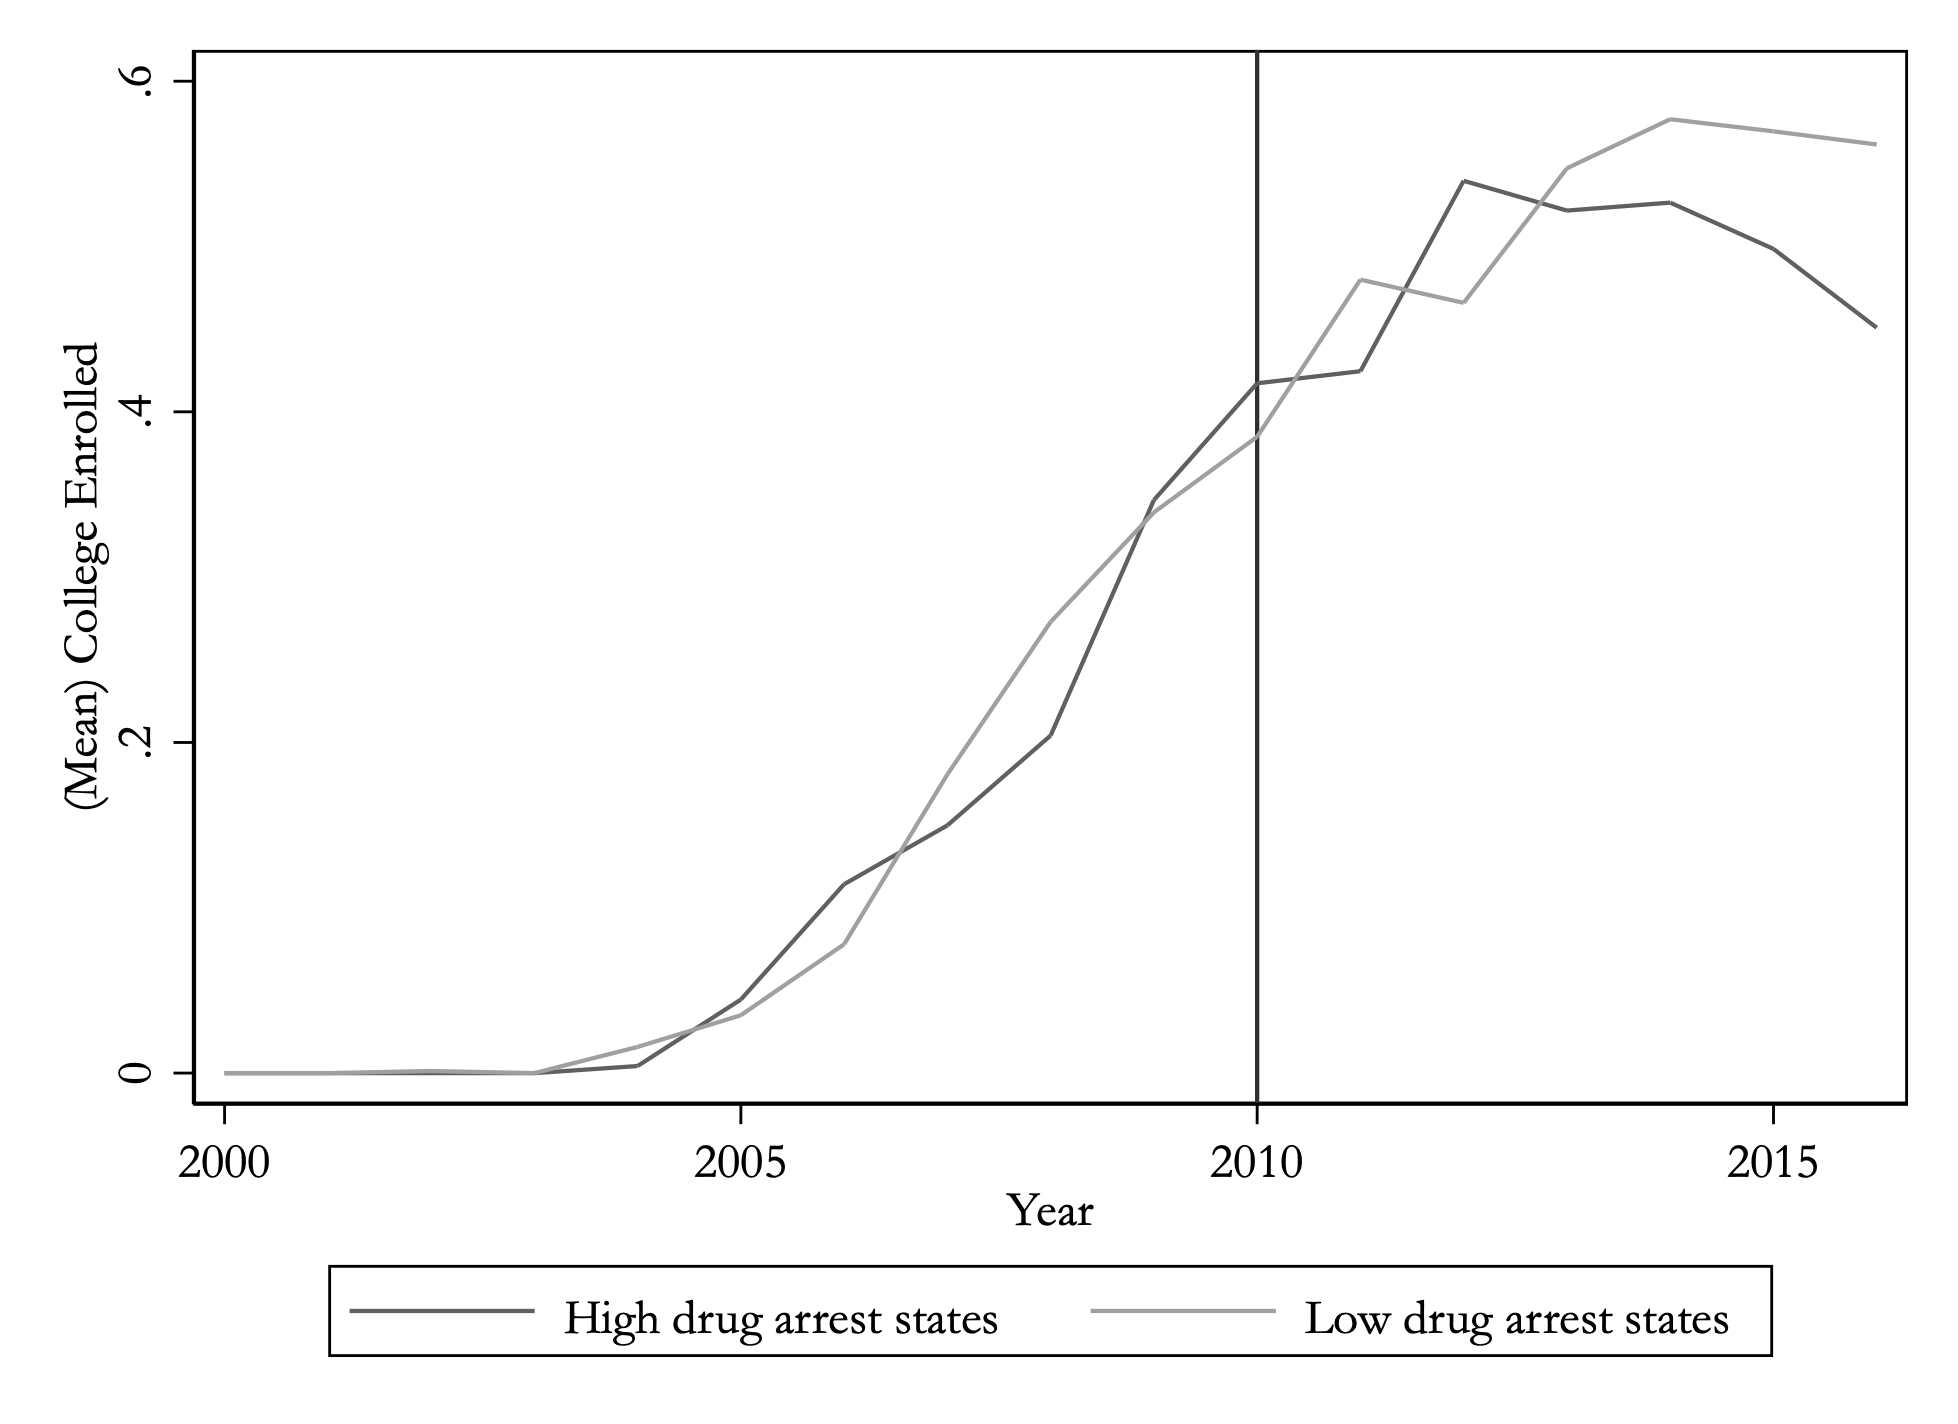
\includegraphics[width=7cm]{pretrends/2010/college_enroll_bydrugarrests_jb_2010.png} }}%
    \label{fig:raw_college_highlowjb_1986}%
  \end{figure}
  
  \begin{footnotesize}
    \noindent Note: These figures report the proportion enrolled in college plotted over time using CPS data from 1984-1992 and 2005-2016 for high black adult/juvenile drug arrest states and low black adult/juvenile drug arrest states, where high black adult/juvenile drug arrest states are defined to be those above the 75th percentile in 1984 and 2008. A vertical line is drawn to denote the passage of the Anti-Drug Abuse Act of 1986 and the Fair Sentencing Act of 2010. The sample is defined as black males aged 18-24 in 1986 and 2010 who were not incarcerated at the time of the survey.
  \end{footnotesize}
  
  \clearpage

  % Arrest rate pretrends

  \begin{figure}[h]
    \centering
    \caption{Adult Black Arrest Rate Per 100,000}%
    \subfloat[\centering 1986]{{\includegraphics[width=7cm]{pretrends/1986/ab.png} }}%
    \qquad
    \subfloat[\centering 2010]{{\includegraphics[width=7cm]{pretrends/2010/ab.png} }}%
    \label{fig:raw_ab}%
  \end{figure}
  \begin{figure}[h]
    \centering
    \caption{Juvenile Black Arrest Rate Per 100,000}%
    \subfloat[\centering 1986]{{\includegraphics[width=7cm]{pretrends/1986/ab.png} }}%
    \qquad
    \subfloat[\centering 2010]{{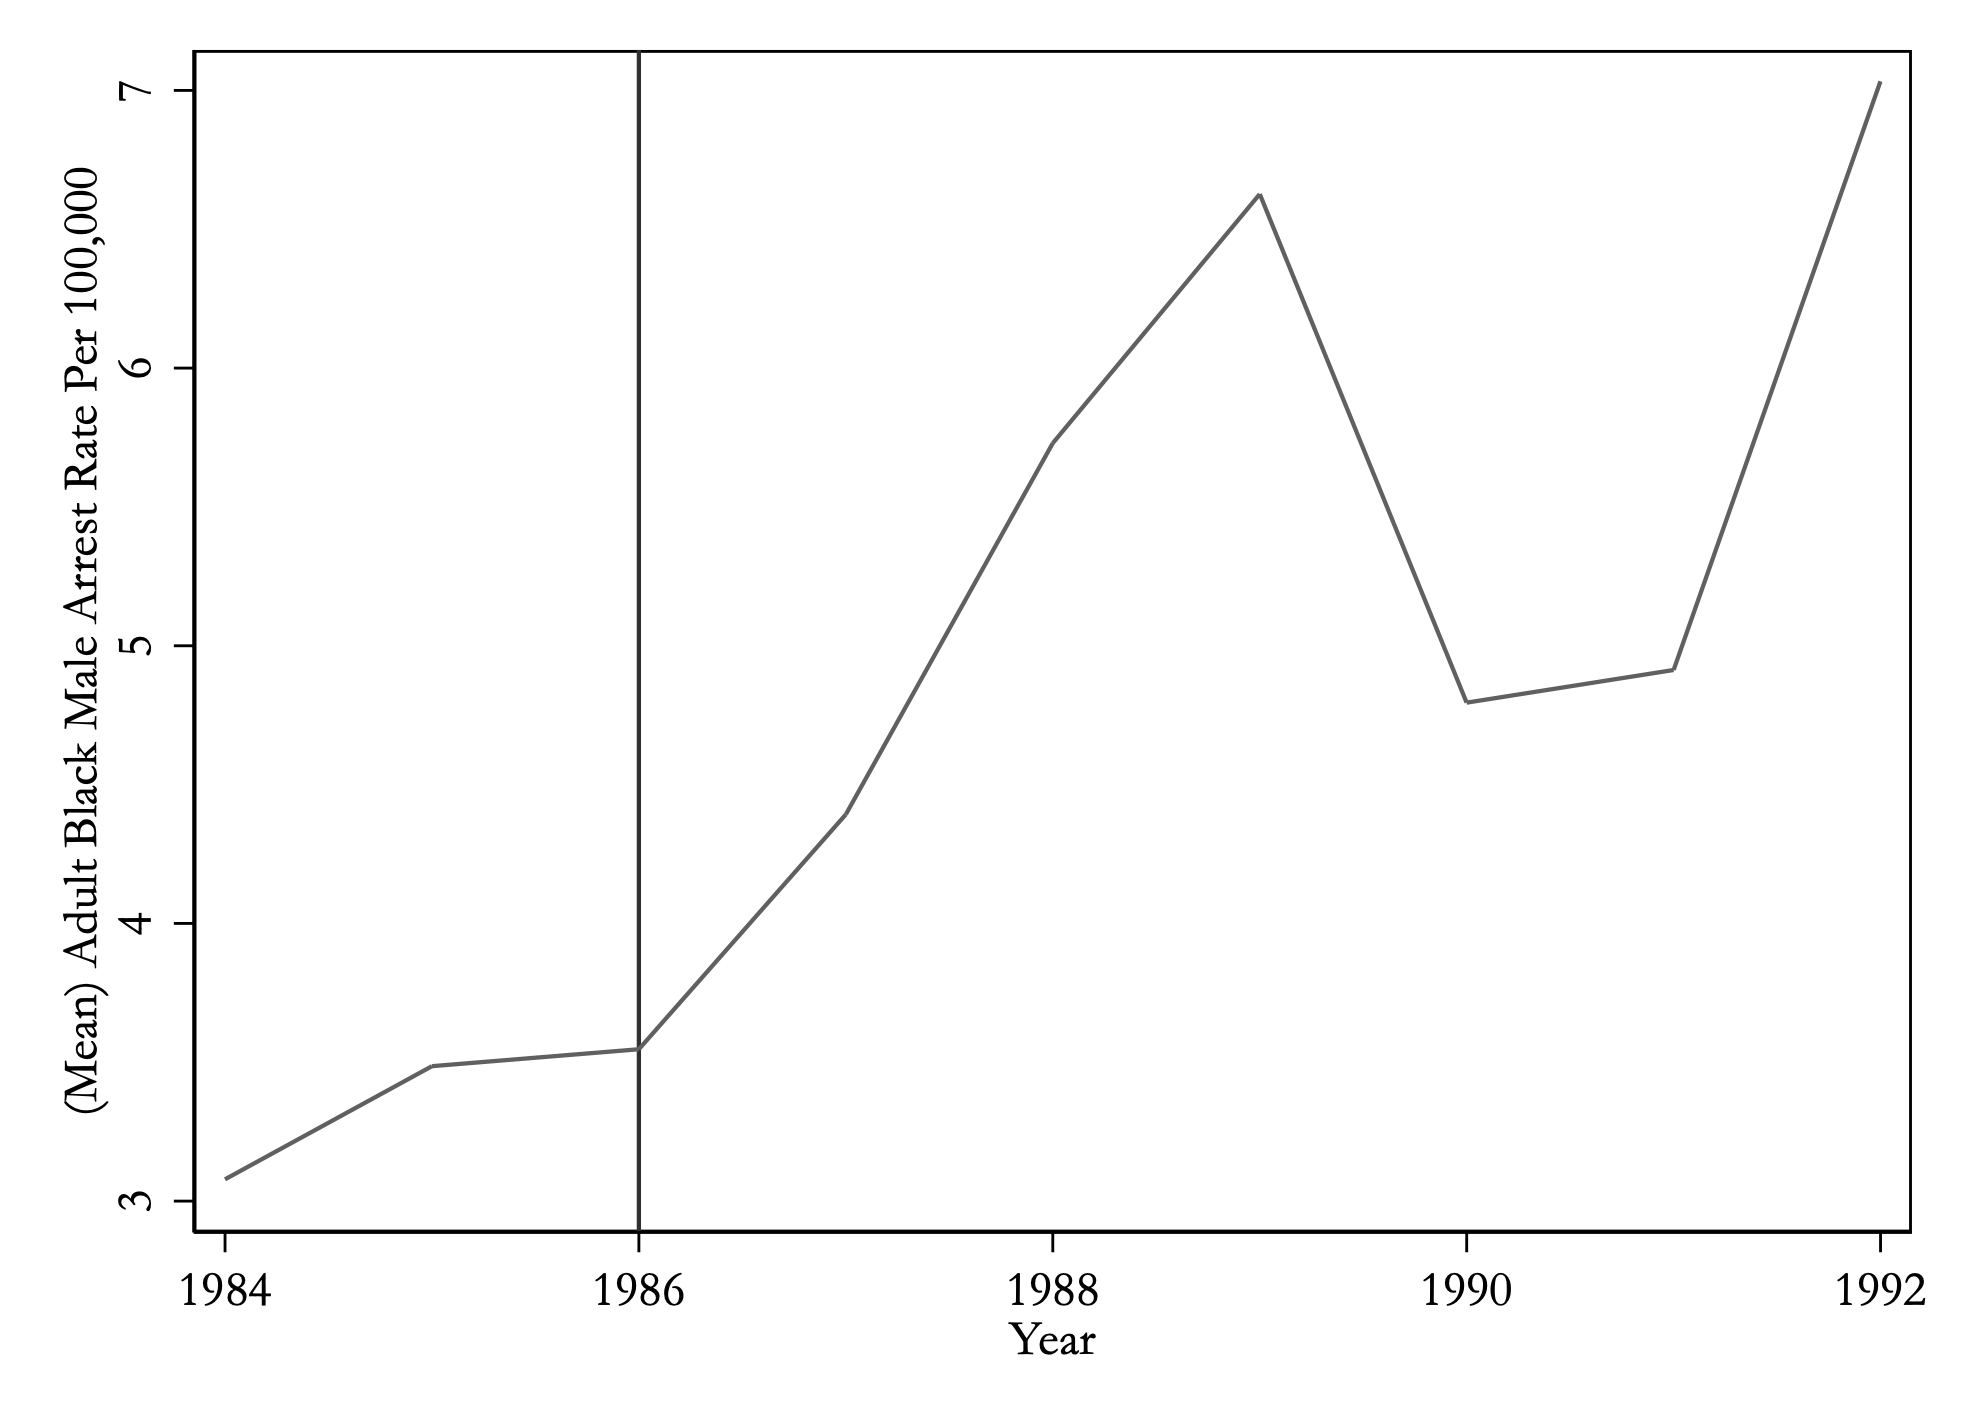
\includegraphics[width=7cm]{pretrends/2010/jb.png} }}%
    \label{fig:raw_jb}%
  \end{figure}

  \begin{footnotesize}
    \noindent Note: These figures report the drug crime arrest rate per 100,000 for black adults and black juveniles separately over time using CPS-UCR merged data from 1984-1992 and 2005-2016. A vertical line is drawn to denote the passage of the Anti-Drug Abuse Act of 1986 and the Fair Sentencing Act of 2010.
  \end{footnotesize}

  \clearpage

% 1986 pretrends

\begin{figure}[h]
    \centering
    \caption{College Enrollment Around 1984}%
    \subfloat[\centering By race]{{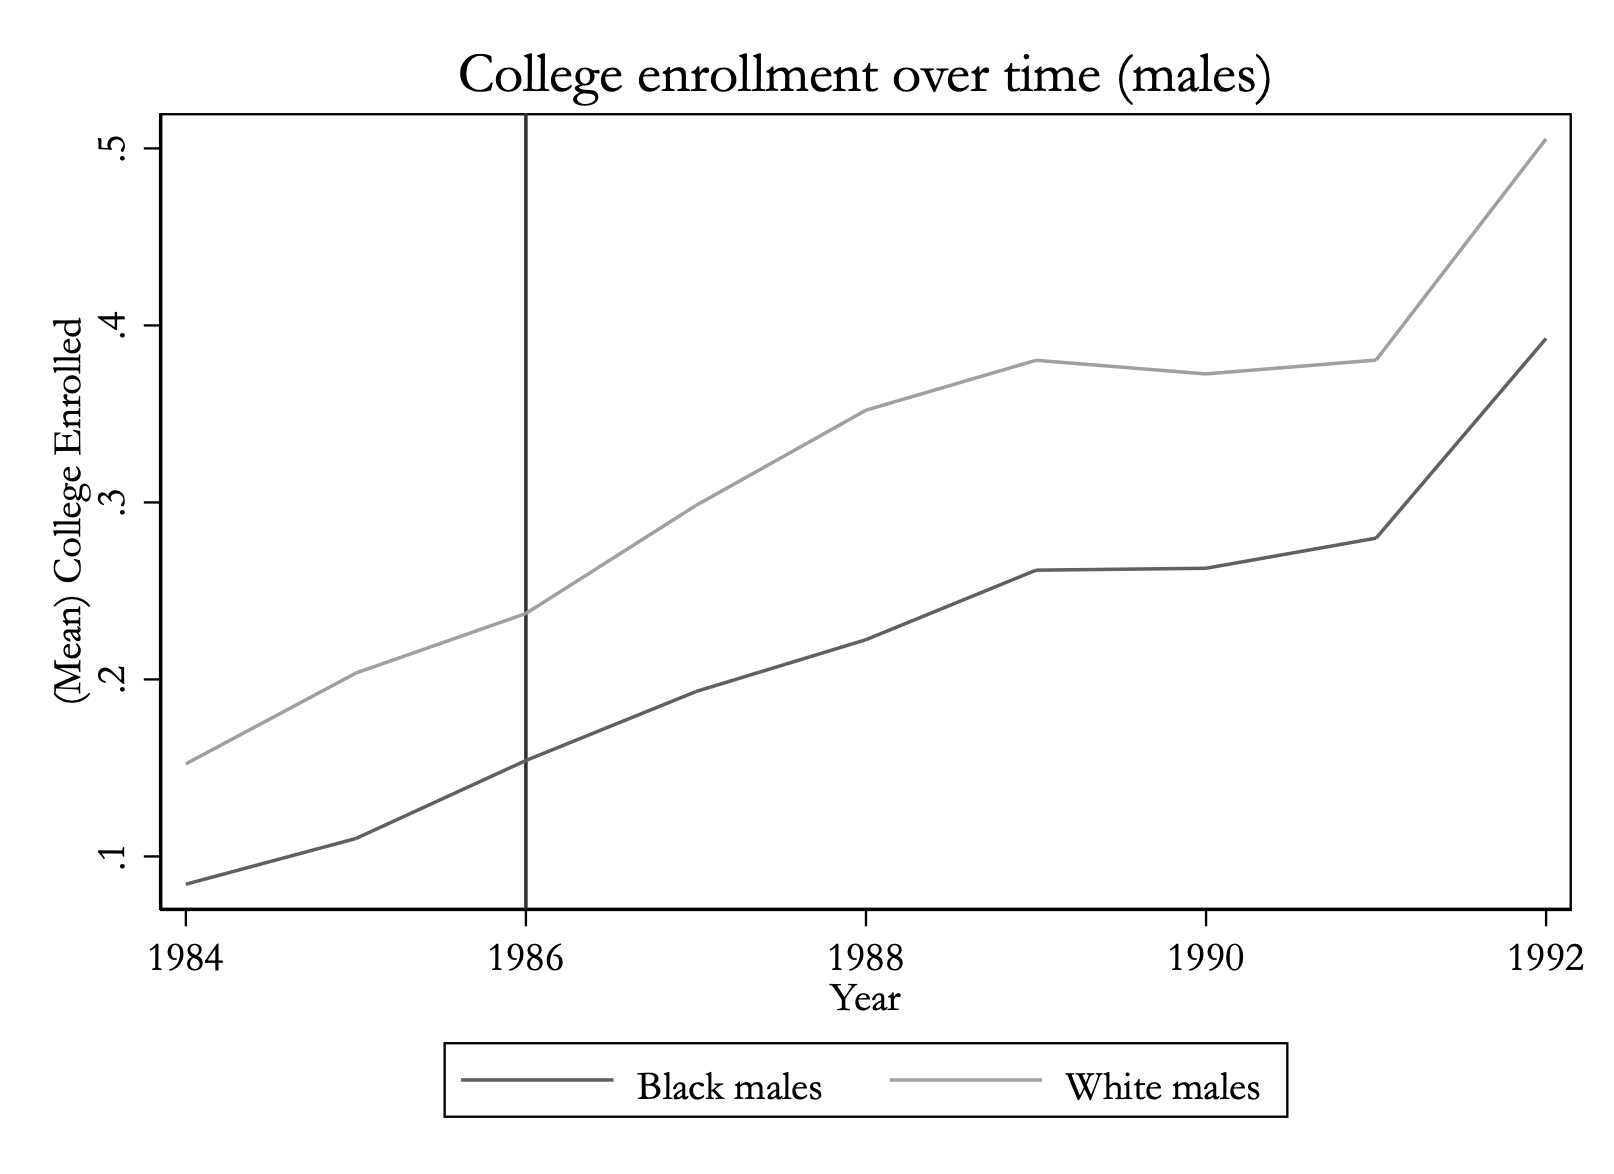
\includegraphics[width=7cm]{pretrends/1986/college_enroll_byrace_1986.png} }}%
    \qquad
    \subfloat[\centering By sex]{{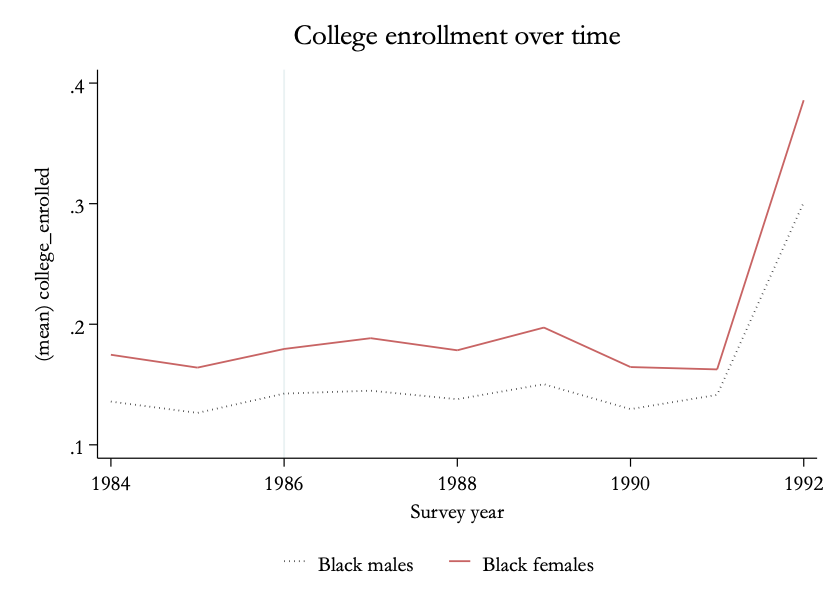
\includegraphics[width=7cm]{pretrends/1986/college_enroll_bysex_1986.png} }}%
    \label{fig:raw_college_1986}%
  \end{figure}
  
  \begin{figure}[h]
    \centering
    \caption{Family Income Around 1984}%
    \subfloat[\centering By race]{{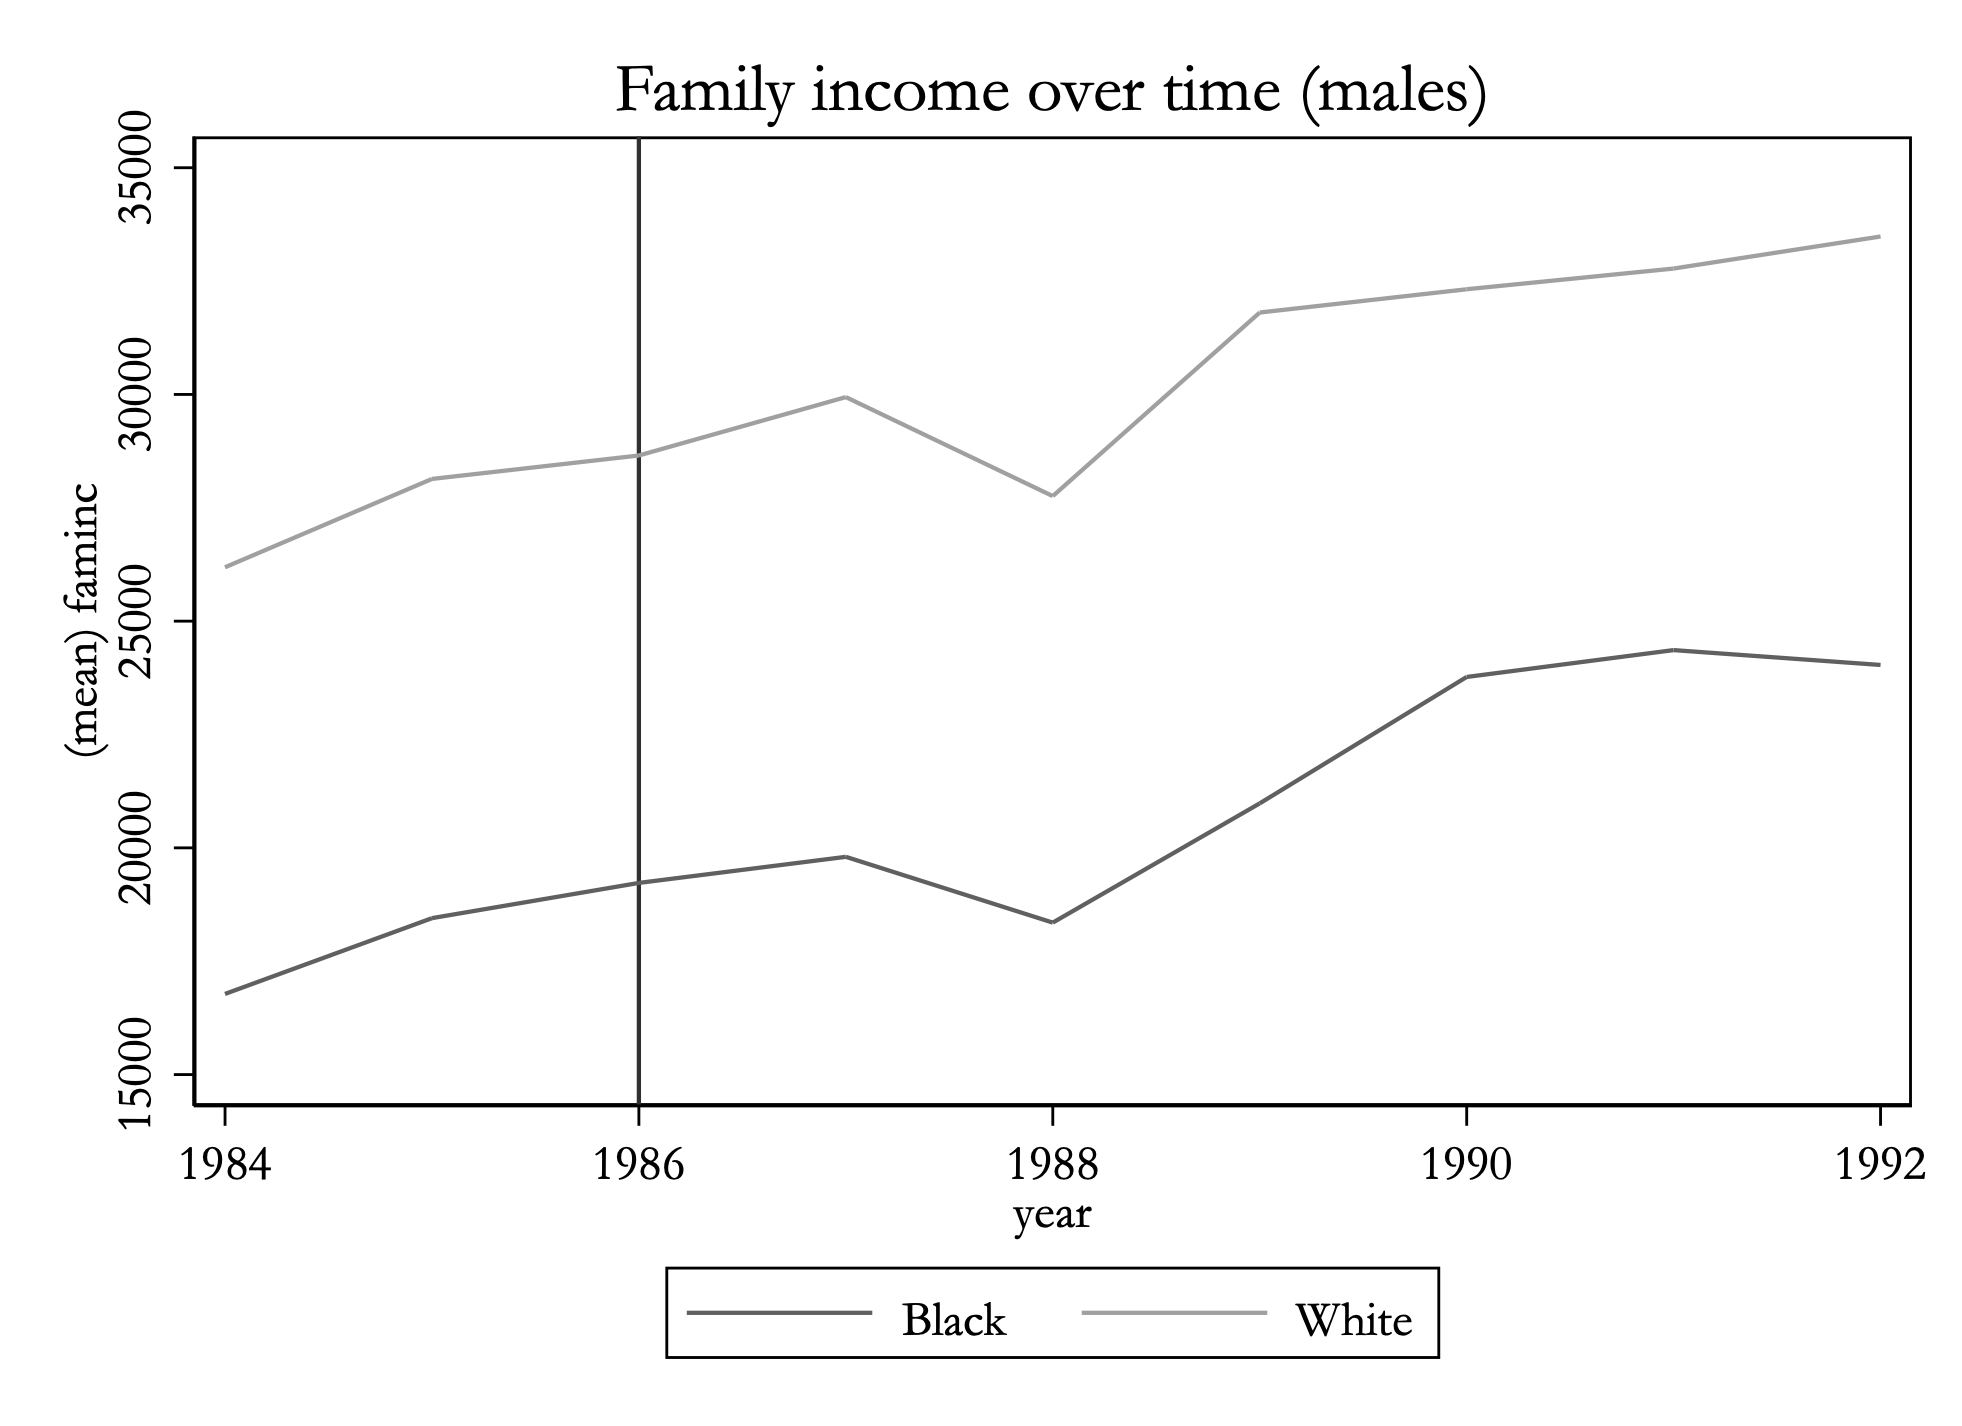
\includegraphics[width=7cm]{pretrends/1986/faminc_byrace_1986.png} }}%
    \qquad
    \subfloat[\centering By sex]{{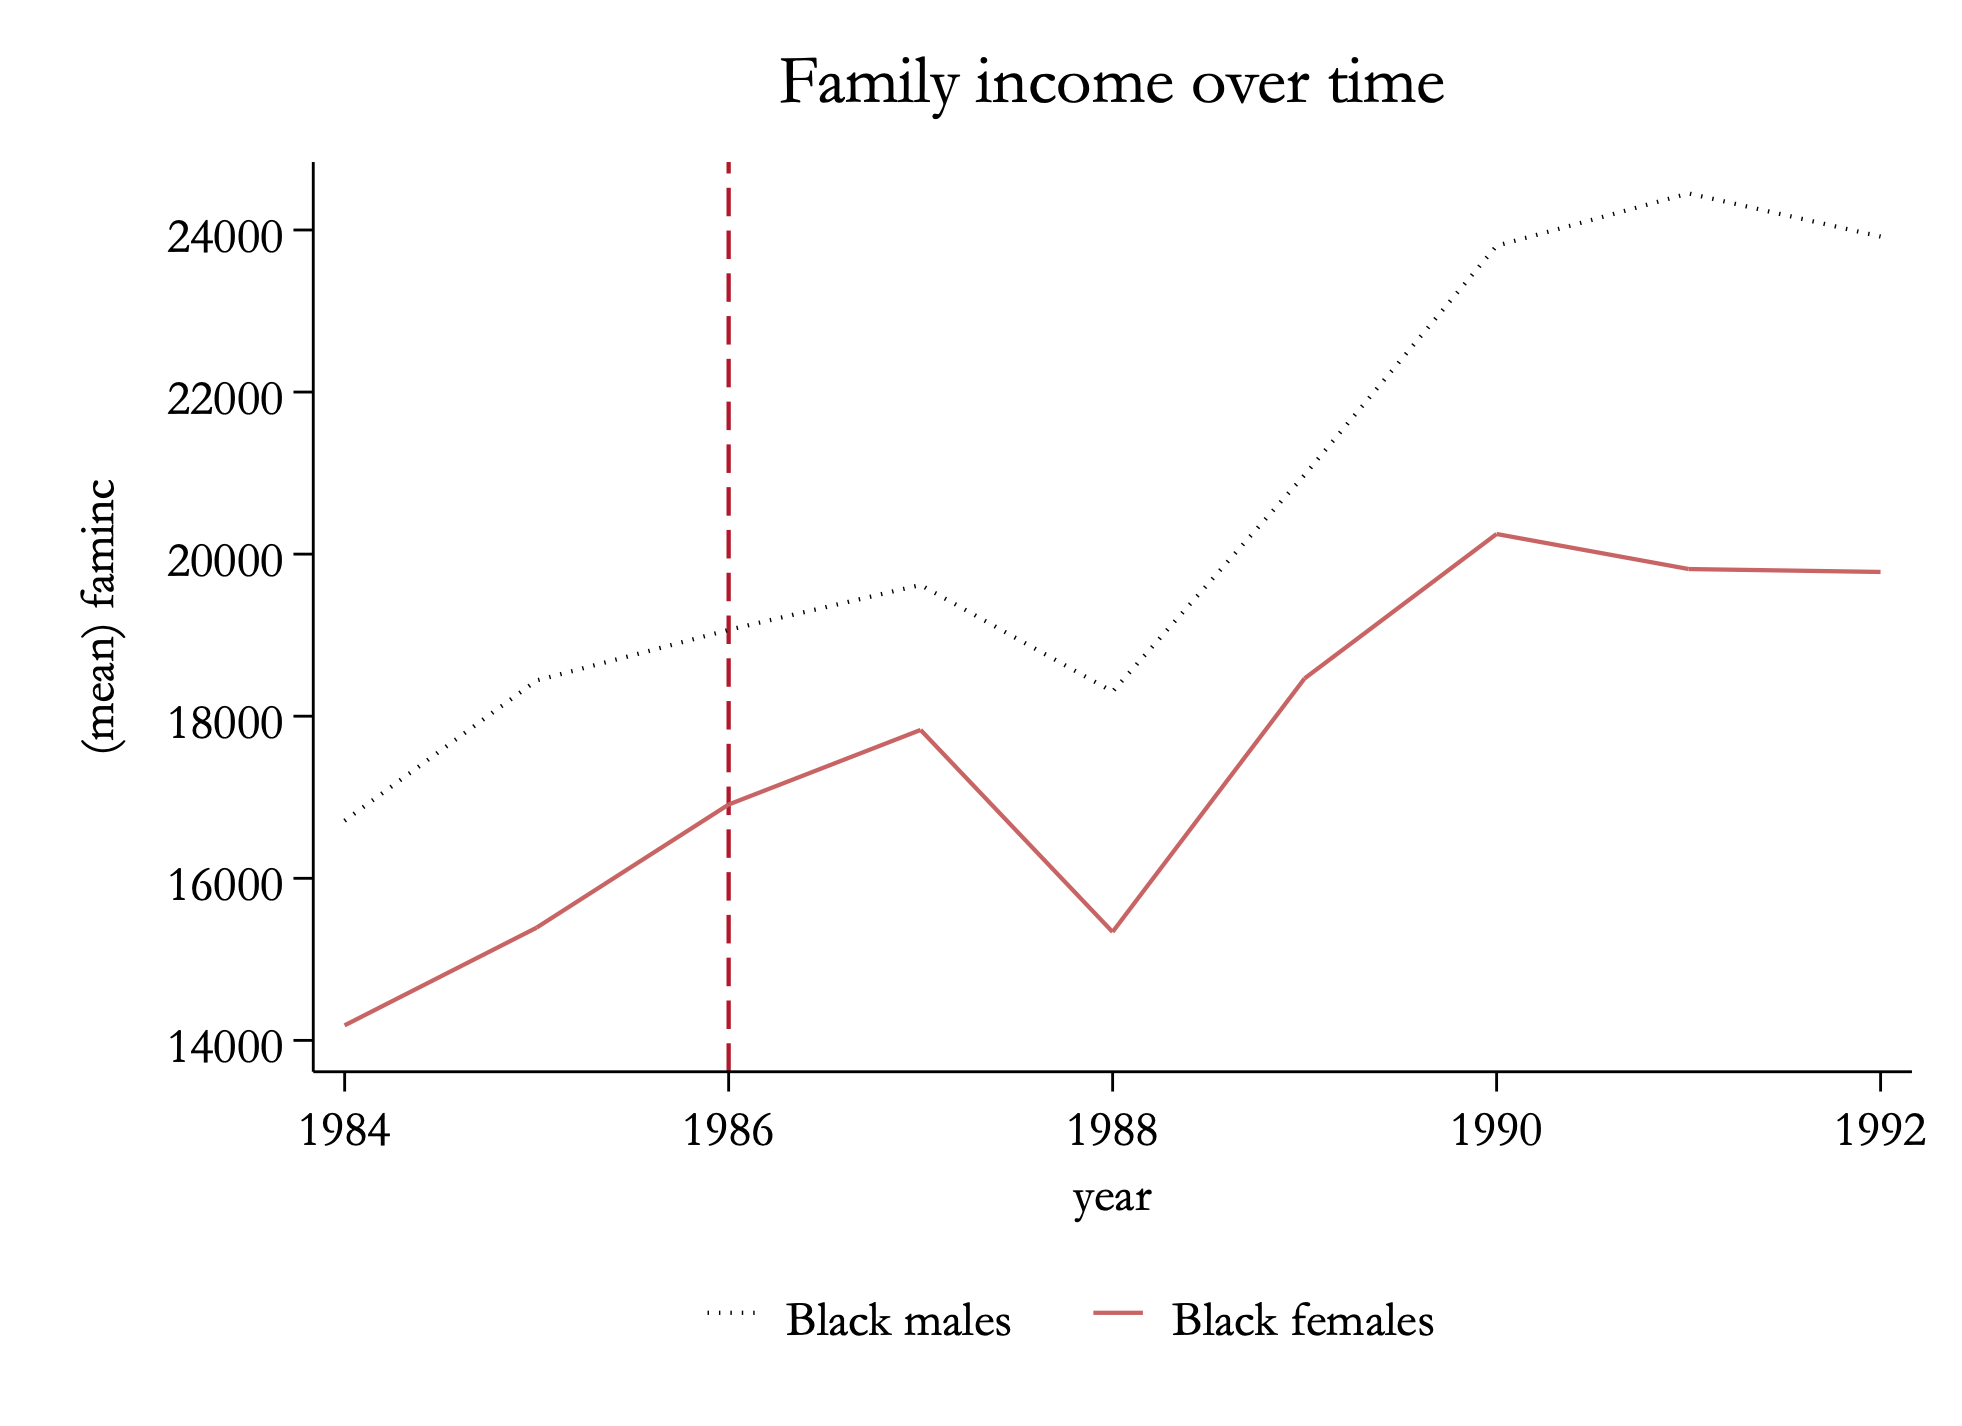
\includegraphics[width=7cm]{pretrends/1986/faminc_bysex_1986.png} }}%
    \label{fig:raw_faminc_1986}%
  \end{figure}
  
  \begin{footnotesize}
    \noindent Note: These figures report the outcomes for various subgroups plotted over time using CPS data from 1984-1992. Figure \ref{fig:raw_college_1986} reports the proportion enrolled in college, while figure \ref{fig:raw_faminc_1986} reports the average family income. A vertical line is drawn to denote the passage of the Anti-Drug Abuse Act of 1986. The universe of samples is defined as participants aged 18-24 in 1986 who were not incarcerated at the time of the survey.
  \end{footnotesize}
  
  \clearpage
  
  % 2010 pretrends
  
  \begin{figure}[h]
    \centering
    \caption{College Enrollment Around 2010}%
    \subfloat[\centering By race]{{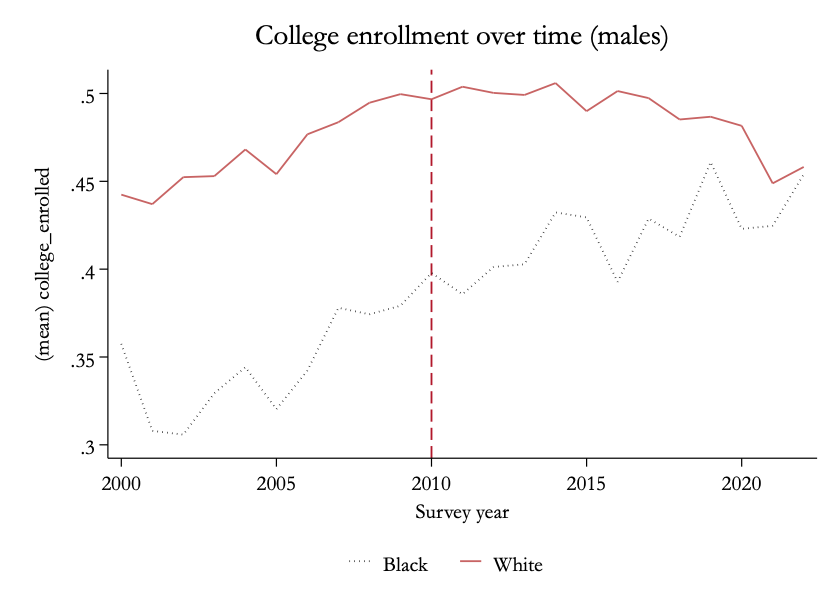
\includegraphics[width=7cm]{pretrends/2010/college_enroll_byrace_2010.png} }}%
    \qquad
    \subfloat[\centering By sex]{{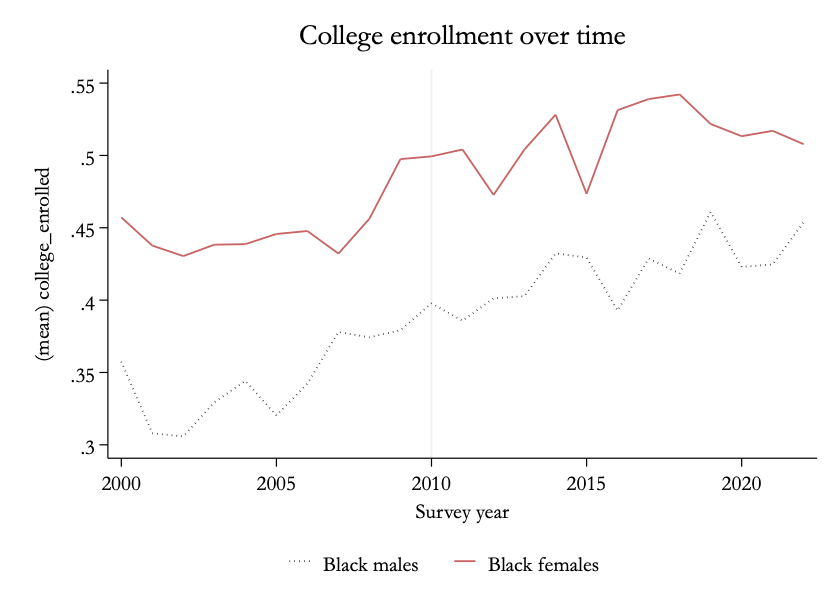
\includegraphics[width=7cm]{pretrends/2010/college_enroll_bysex_2010.png} }}%
    \label{fig:raw_college_2010}%
  \end{figure}
  
  \begin{figure}[h]
    \centering
    \caption{Family Income Around 2010}%
    \subfloat[\centering By race]{{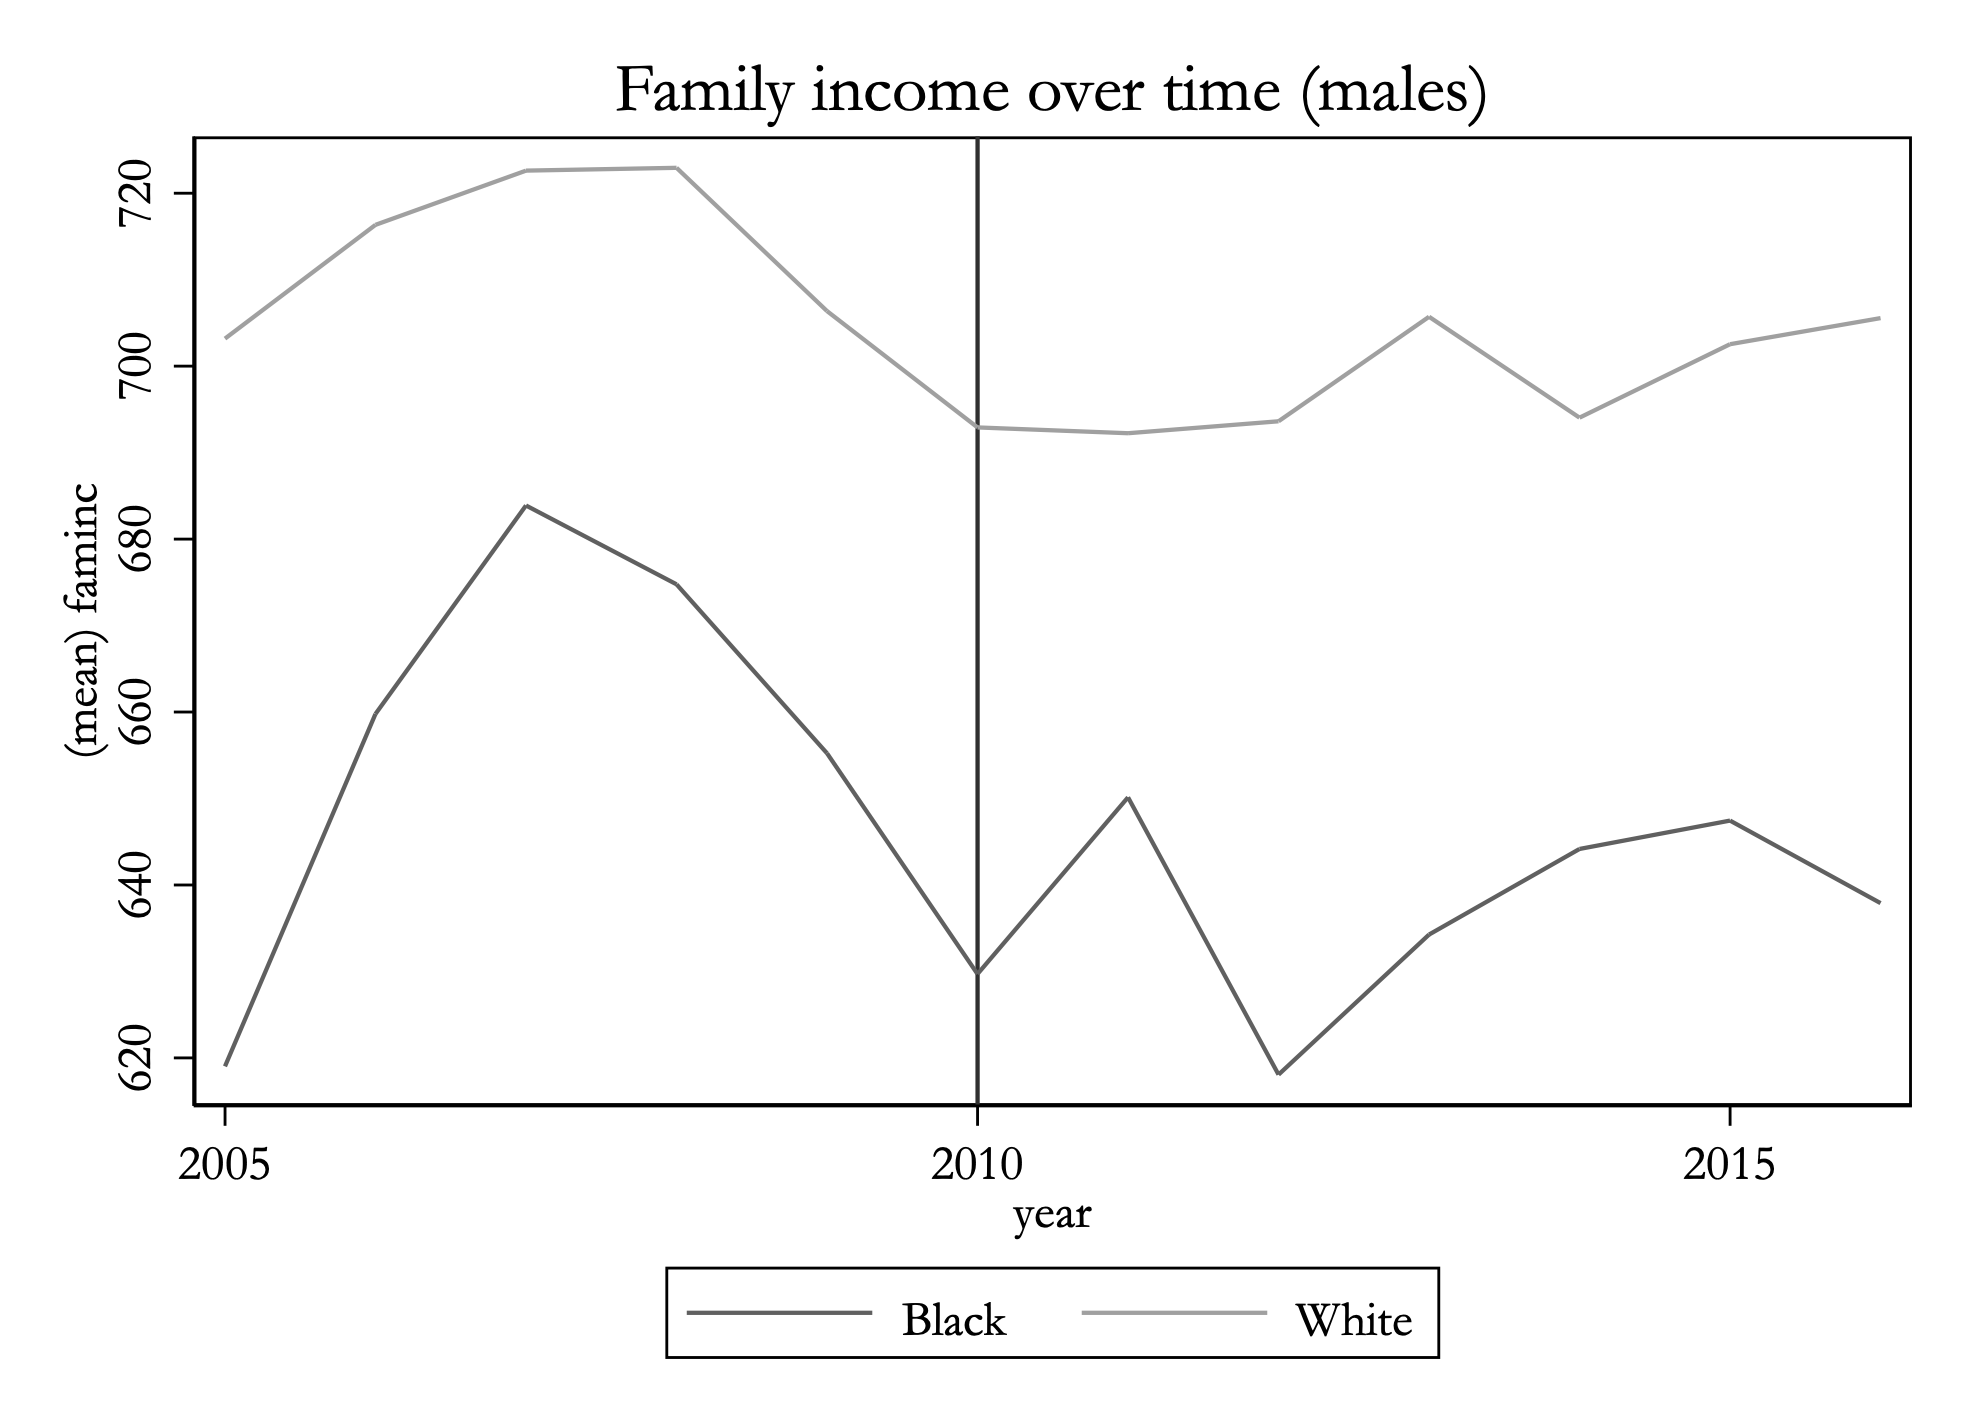
\includegraphics[width=7cm]{pretrends/2010/faminc_byrace_2010.png} }}%
    \qquad
    \subfloat[\centering By sex]{{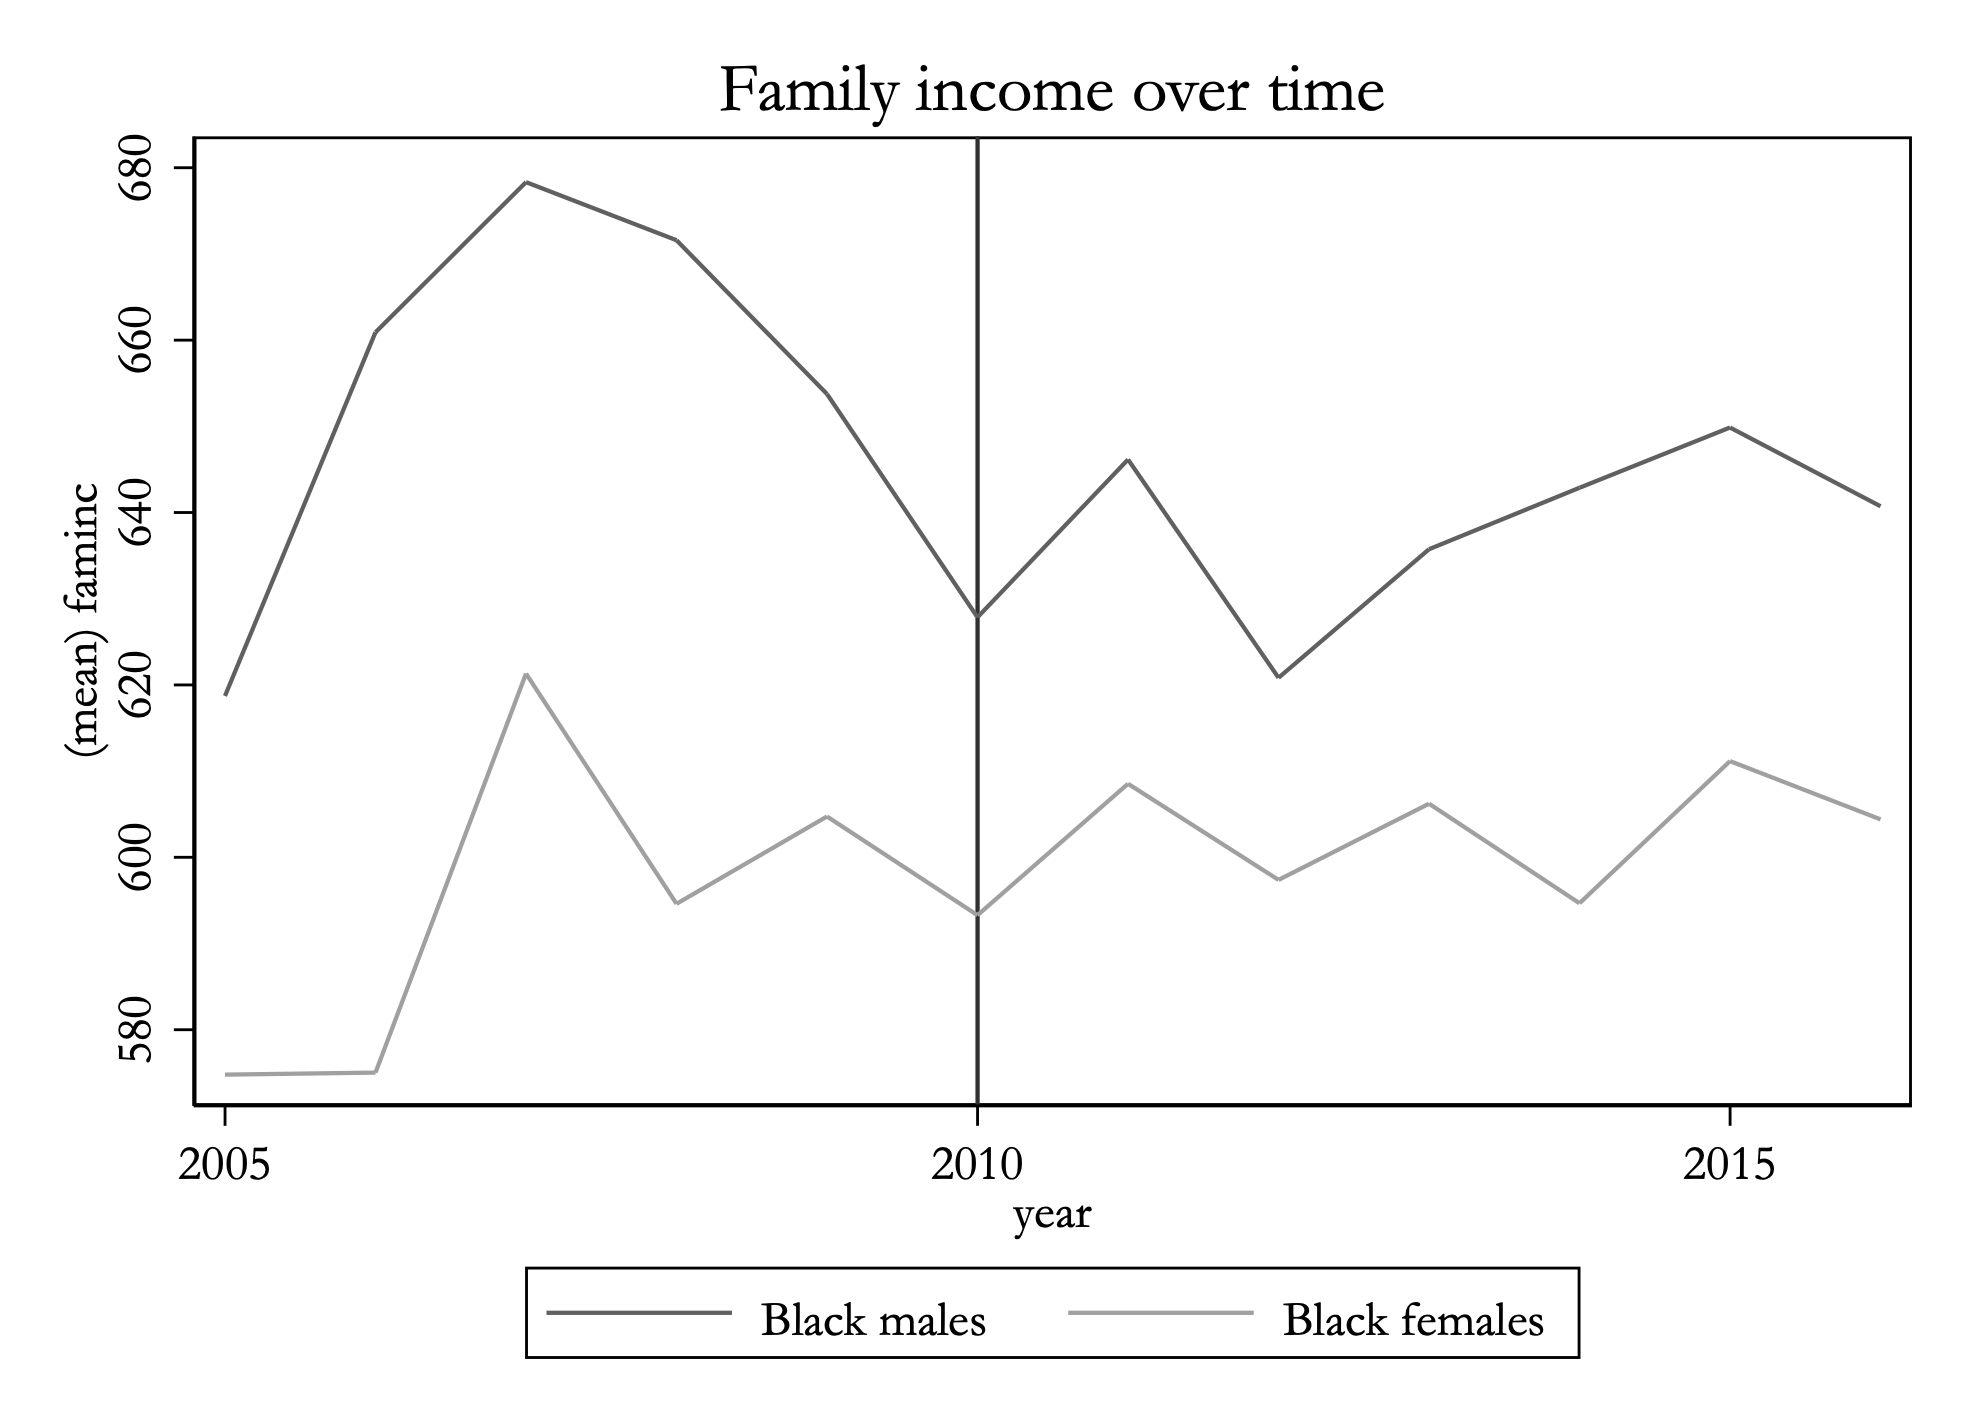
\includegraphics[width=7cm]{pretrends/2010/faminc_bysex_2010.png} }}%
    \label{fig:raw_faminc_2010}%
  \end{figure}
  
  \begin{footnotesize}
    \noindent Note: These figures report the outcomes for various subgroups plotted over time using CPS data from 2005-2016. Figure \ref{fig:raw_college_2010} reports the proportion enrolled in college, while figure \ref{fig:raw_faminc_2010} reports the average family income. A vertical line is drawn to denote the passage of the Fair Sentencing Act of 2010. The universe of samples is defined as participants aged 18-24 in 2010 who were not incarcerated at the time of the survey.
  \end{footnotesize}
  
  \clearpage
  
  \begin{figure}[h]
    \caption{Effect of Anti-Drug Abuse Act on Drug-related Arrest Rate of Adult Black Men, Comparing States with High and Low Black Adult Drug-Related Arrest Rates}
    \centering
    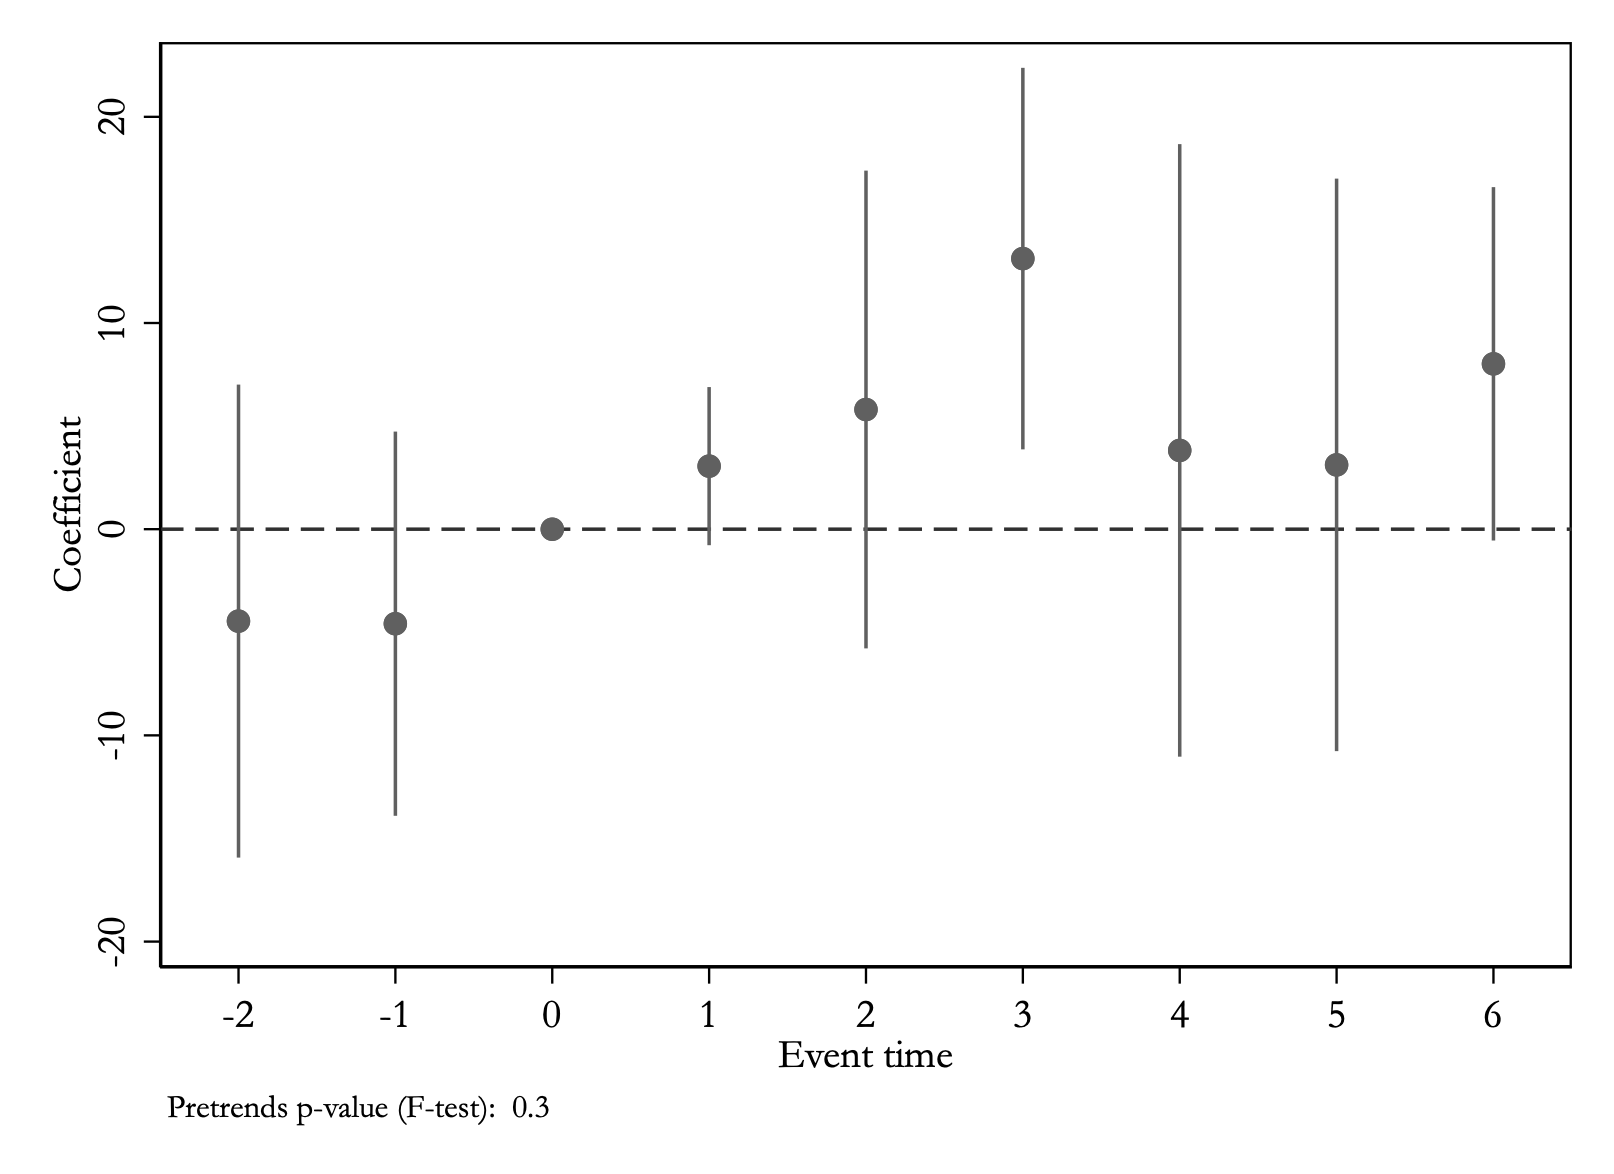
\includegraphics[width=1\textwidth]{eventstudy/high_drug_use/high_drug_eventstudy_1986.png}
    \label{fig:ab_es_1986}
  \end{figure}
  
  \begin{footnotesize}
    \noindent Note: This figure reports coefficients from the estimation of equation \ref{eq:state_level_es} evaluating the impact of the Anti-Drug Abuse Act of 1986 on arrest rates per 100,000 related to drug violations using CPS and UCR data from 1982-1992. Event time $0 \coloneqq 1986$. The coefficients represent the change in outcomes for high-drug arrest states relative to non-high-drug arrest states, where high black adult drug arrest states are defined to be those above the 75th percentile in 1984. The sample is defined as black males aged 18-24 in 1986 who were not incarcerated at the time of the survey. Control variables include population and unemployment rates at the state-year level. Right tail arrest rate outliers were winsorizing at the 95\% level.
  \end{footnotesize}
  
  \clearpage
  
  %\begin{figure*}[h]
   % \caption{Pretrends for Event study 1986, AB arrest rate 18F}
   % 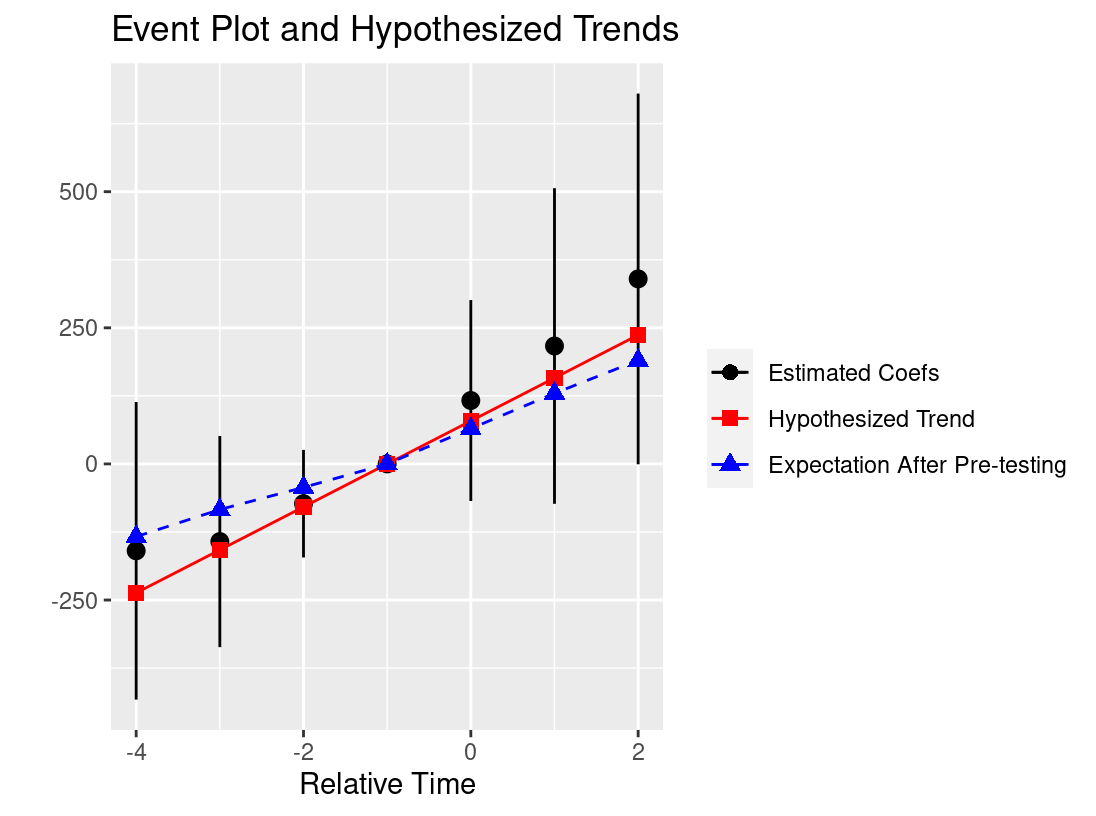
\includegraphics[width=1\textwidth]{roth_test.png}
  %\end{figure*}
  
  %Power: 0.499. Bayes.Factor: 0.550.  Likelihood.Ratio: 2.024
  
  %\clearpage
  
  \begin{figure}[h]
    \caption{Effect of Fair Sentencing Act on Drug-related Arrest Rate of Adult Black Men, Comparing States with High and Low Black Adult Drug-Related Arrest Rate}
    \centering
    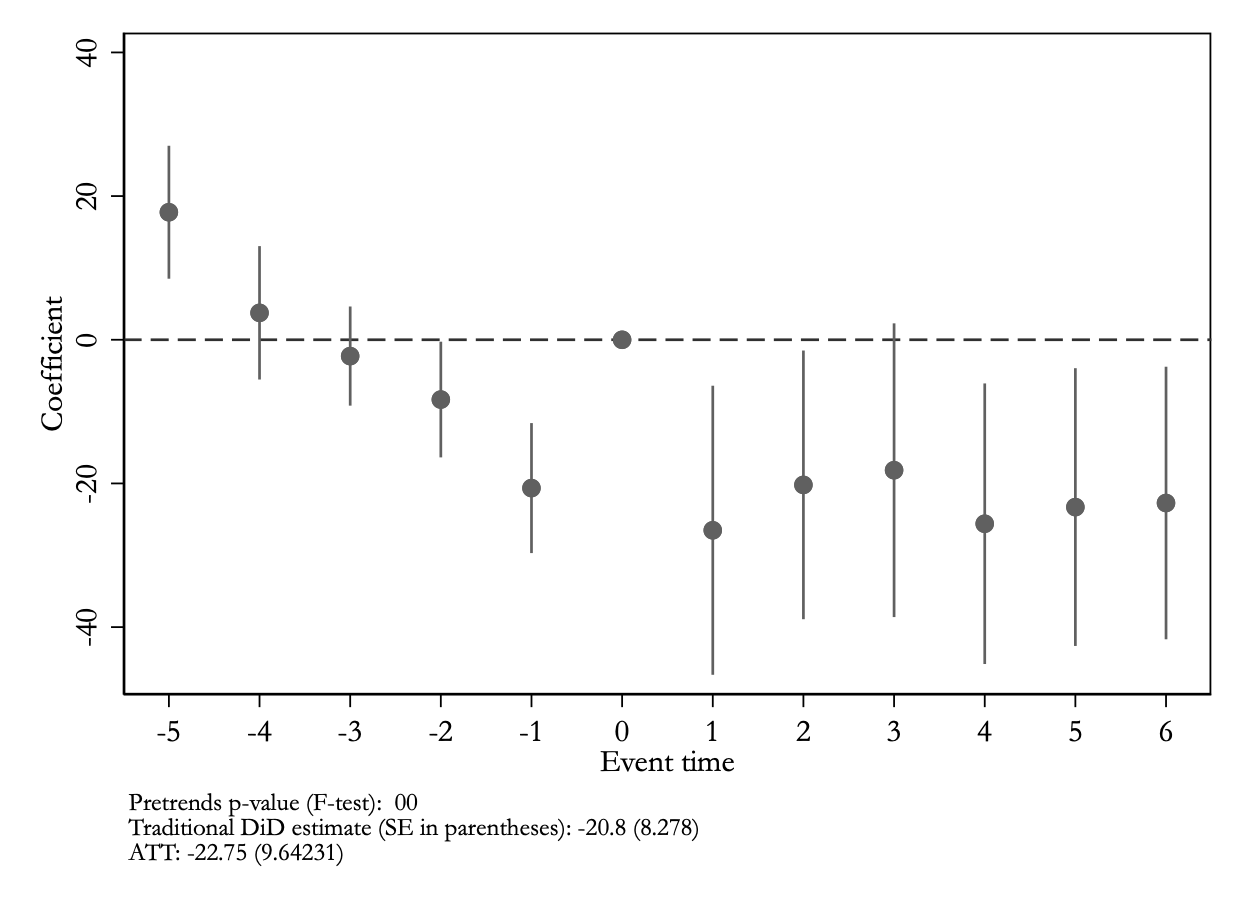
\includegraphics[width=1\textwidth]{eventstudy/high_drug_use/high_drug_eventstudy_2010_ab.png}
    \label{fig:ab_es_2010}
  \end{figure}
  
  \begin{footnotesize}
    \noindent Note: This figure reports coefficients from the estimation of equation 1 evaluating the impact of the Fair Sentencing Act of 2010 on arrest rates per 100,000 related to drug violations using CPS and UCR data from 2005-2015. Event time $0 \coloneqq 2010$. The coefficients represent the change in outcomes for high black adult drug arrest states relative to non-high-drug arrest states, where high-drug arrest states are defined to be those above the 75th percentile in 2008. The sample is defined as black males aged 18-24 in 2010 who were not incarcerated at the time of the survey. Control variables include population and unemployment rates at the state-year level. 
  \end{footnotesize}

\clearpage

  \begin{figure}[h]
    \caption{Effect of Anti-Drug Abuse Act on Drug-related Arrest Rate of Black Men, Comparing States with High and Low Black Juvenile Drug-Related Arrest Rate}
    \centering
    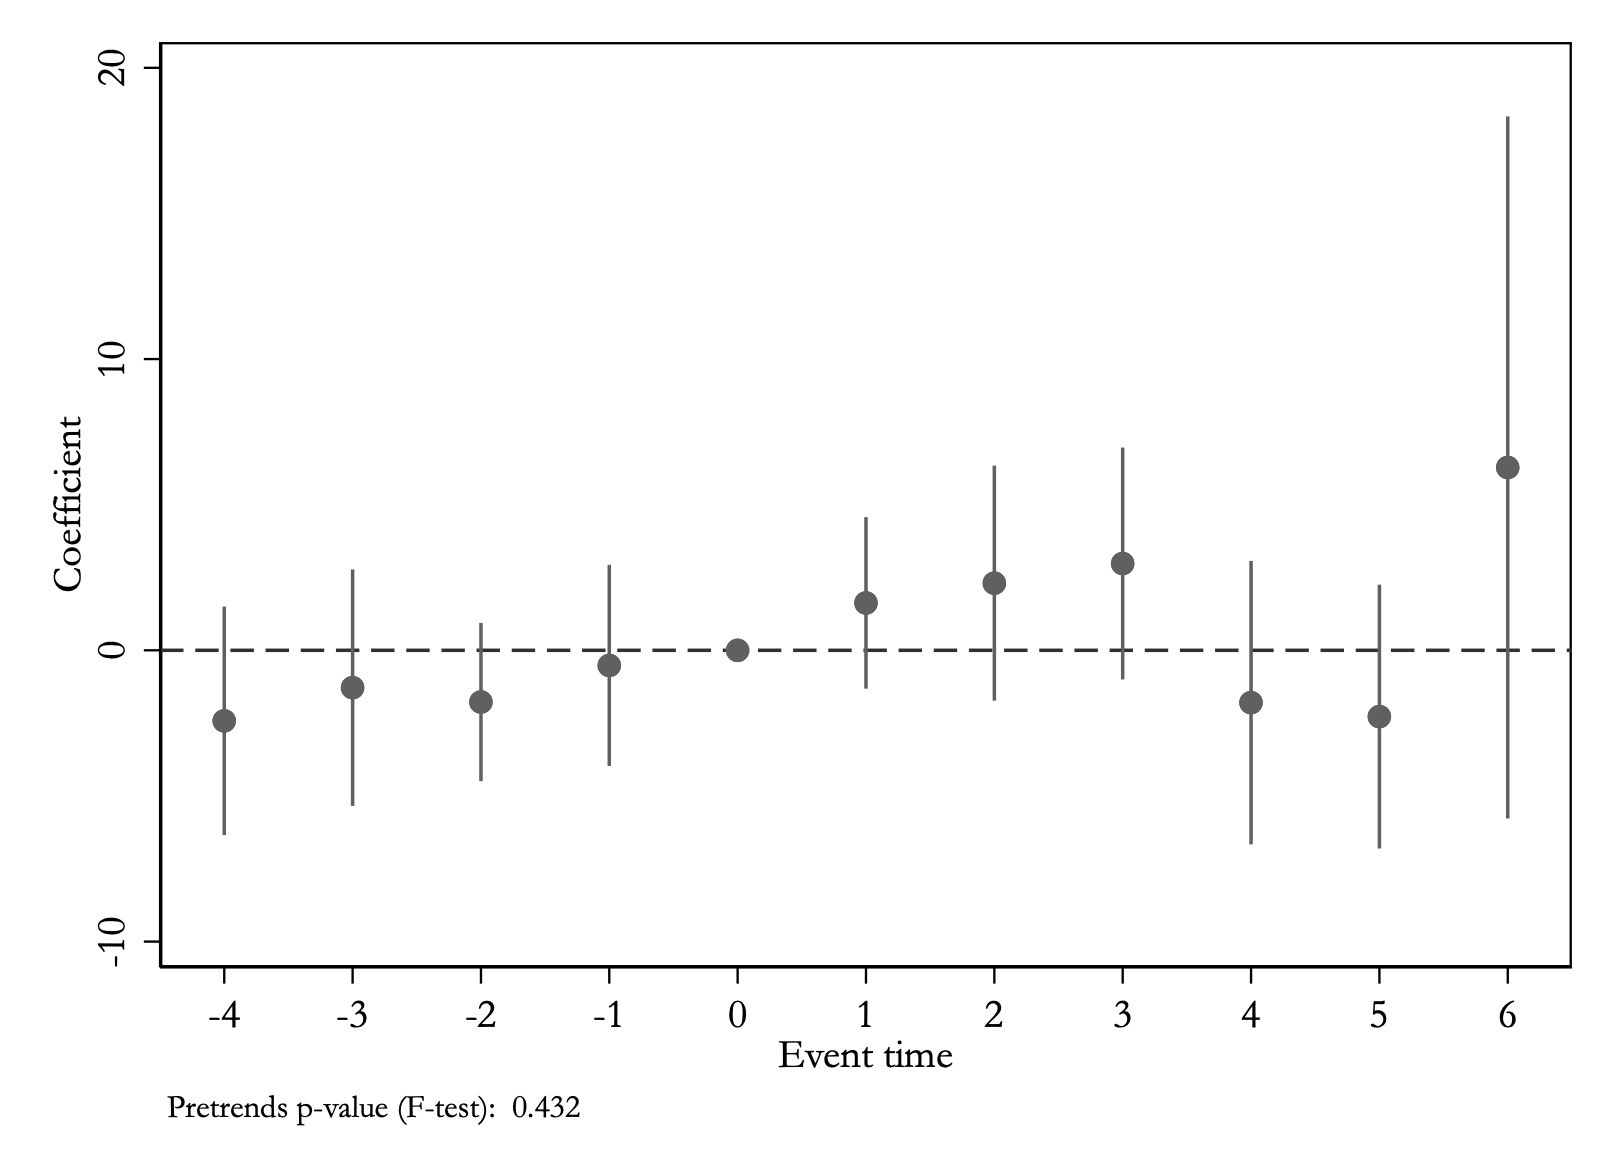
\includegraphics[width=1\textwidth]{eventstudy/high_drug_use/high_drug_eventstudy_1986_jb.png}
    \label{fig:jb_es_1986}
  \end{figure}

  \begin{footnotesize}
    \noindent Note: This figure reports coefficients from the estimation of equation 1 evaluating the impact of the Anti-Drug Abuse Act of 1986 on arrest rates per 100,000 related to drug violations using CPS and UCR data from 1982-1992. Event time $0 \coloneqq 1986$. The coefficients represent the change in outcomes for high black juvenile drug arrest states relative to non-high-drug arrest states, where high-drug arrest states are defined to be those above the 75th percentile in 1984. The sample is defined as black males aged 18-24 in 1986 who were not incarcerated at the time of the survey. Control variables include population and unemployment rates at the state-year level. 
  \end{footnotesize}

\clearpage

\begin{figure}[h]
    \caption{Effect of Fair Sentencing Act on Drug-related Arrest Rate of Juvenile Black Men, Comparing States with High and Low Black Juvenile Drug-Related Arrest Rate}
    \centering
    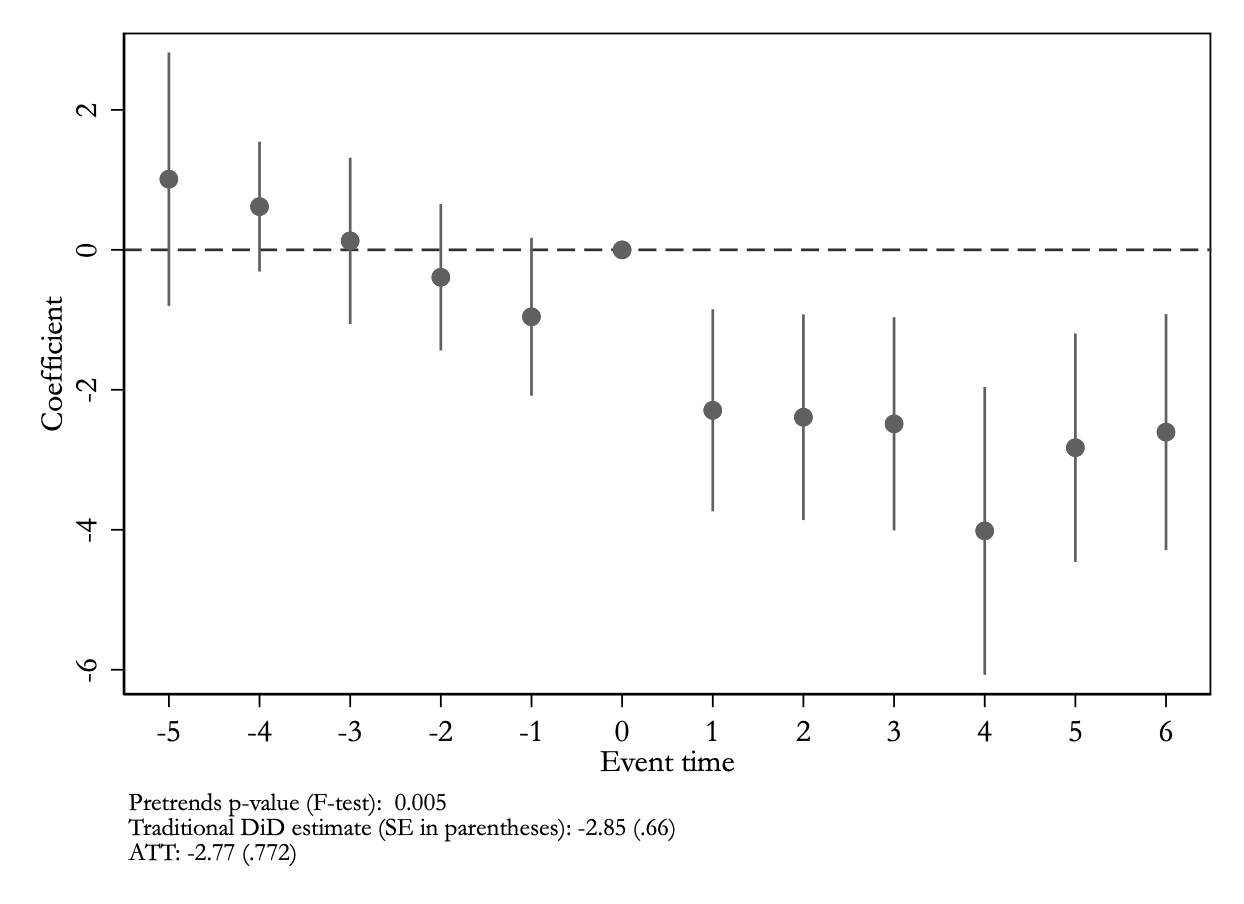
\includegraphics[width=1\textwidth]{eventstudy/high_drug_use/high_drug_eventstudy_2010_jb.png}
    \label{fig:jb_es_2010}
  \end{figure}

  \begin{footnotesize}
    \noindent Note: This figure reports coefficients from the estimation of equation \ref{eq:1} evaluating the impact of the Fair Sentencing act of 2010 on arrest rates per 100,000 related to drug violations using CPS and UCR data from 2005-2015. Event time $0 \coloneqq 2010$. The coefficients represent the change in outcomes for high black juvenile drug arrest states relative to non-high-drug arrest states, where high-drug arrest states are defined to be those above the 75th percentile in 2008. The sample is defined as black males aged 18-24 in 2010 who were not incarcerated at the time of the survey. Control variables include population and unemployment rates at the state-year level. 
  \end{footnotesize}

  \clearpage

  \begin{figure}[h]
    \centering
    \caption{Distribution of Black Juvenile Drug-Related Arrest Rates By State / Year}%
    \subfloat[\centering 1986]{{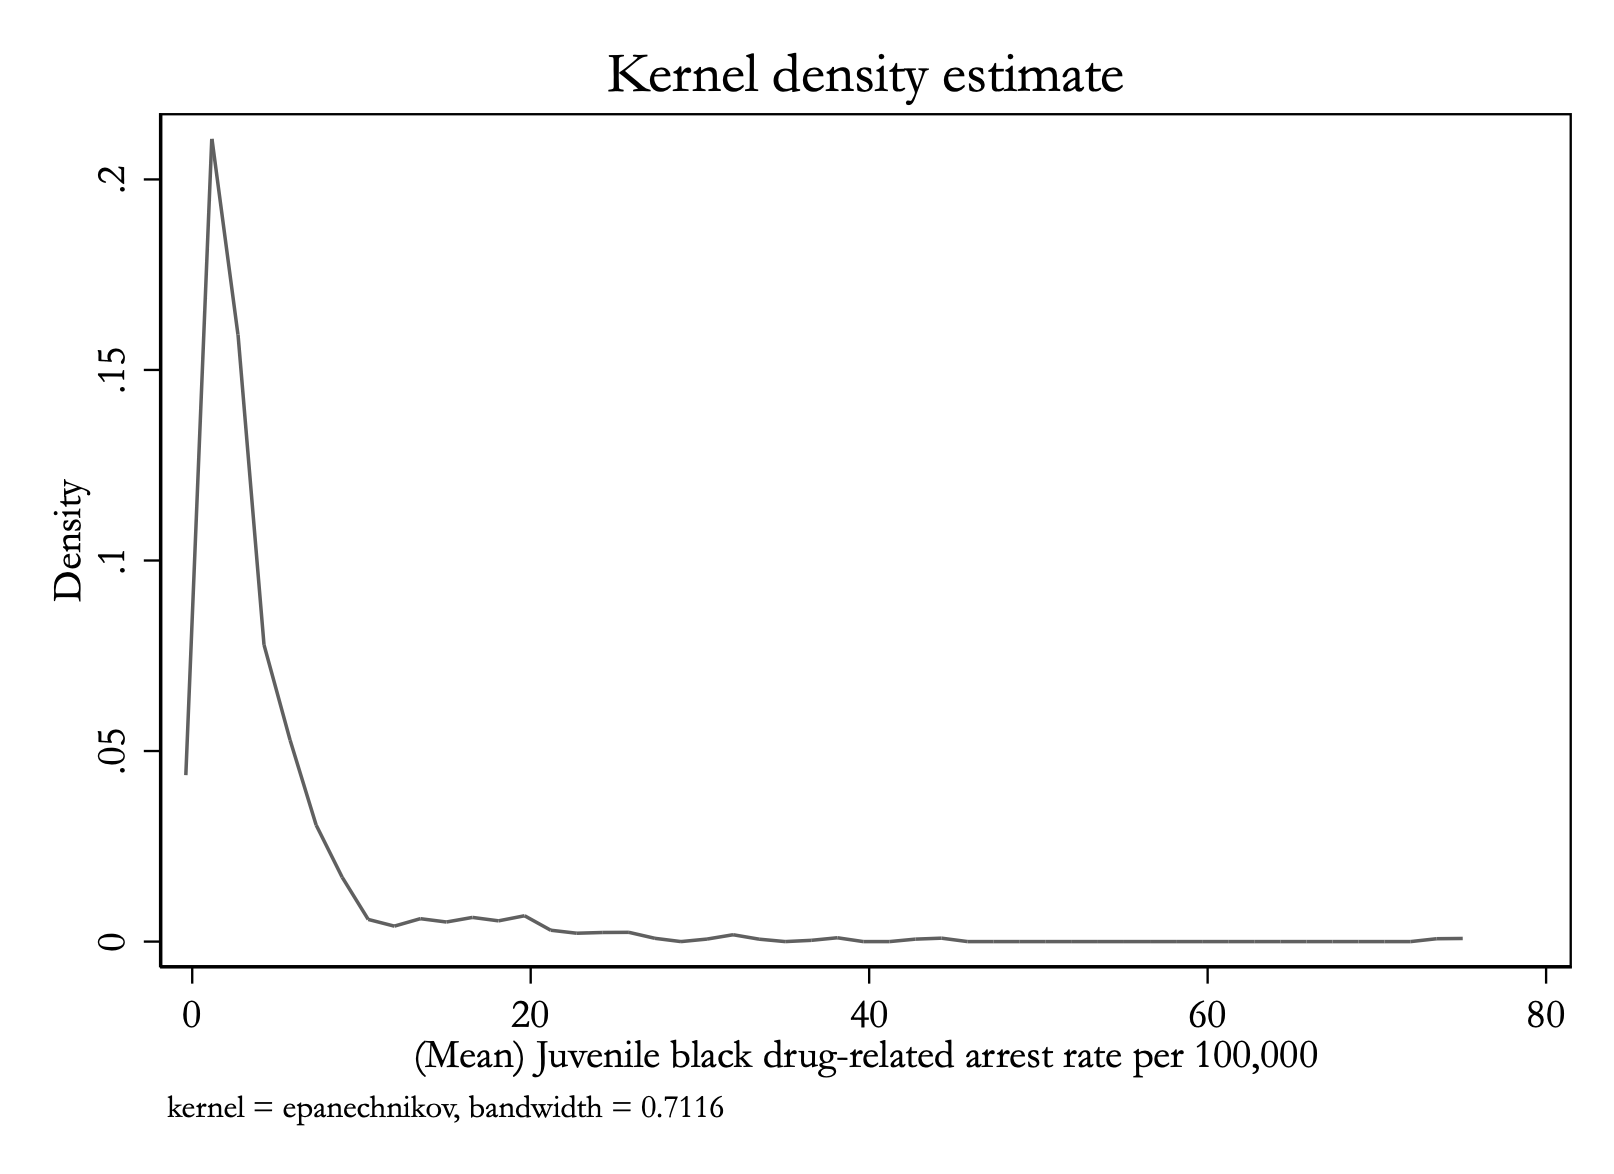
\includegraphics[width=7cm]{descriptive/norm_jb_100000_density_1986} }}%
    \qquad
    \subfloat[\centering 2010]{{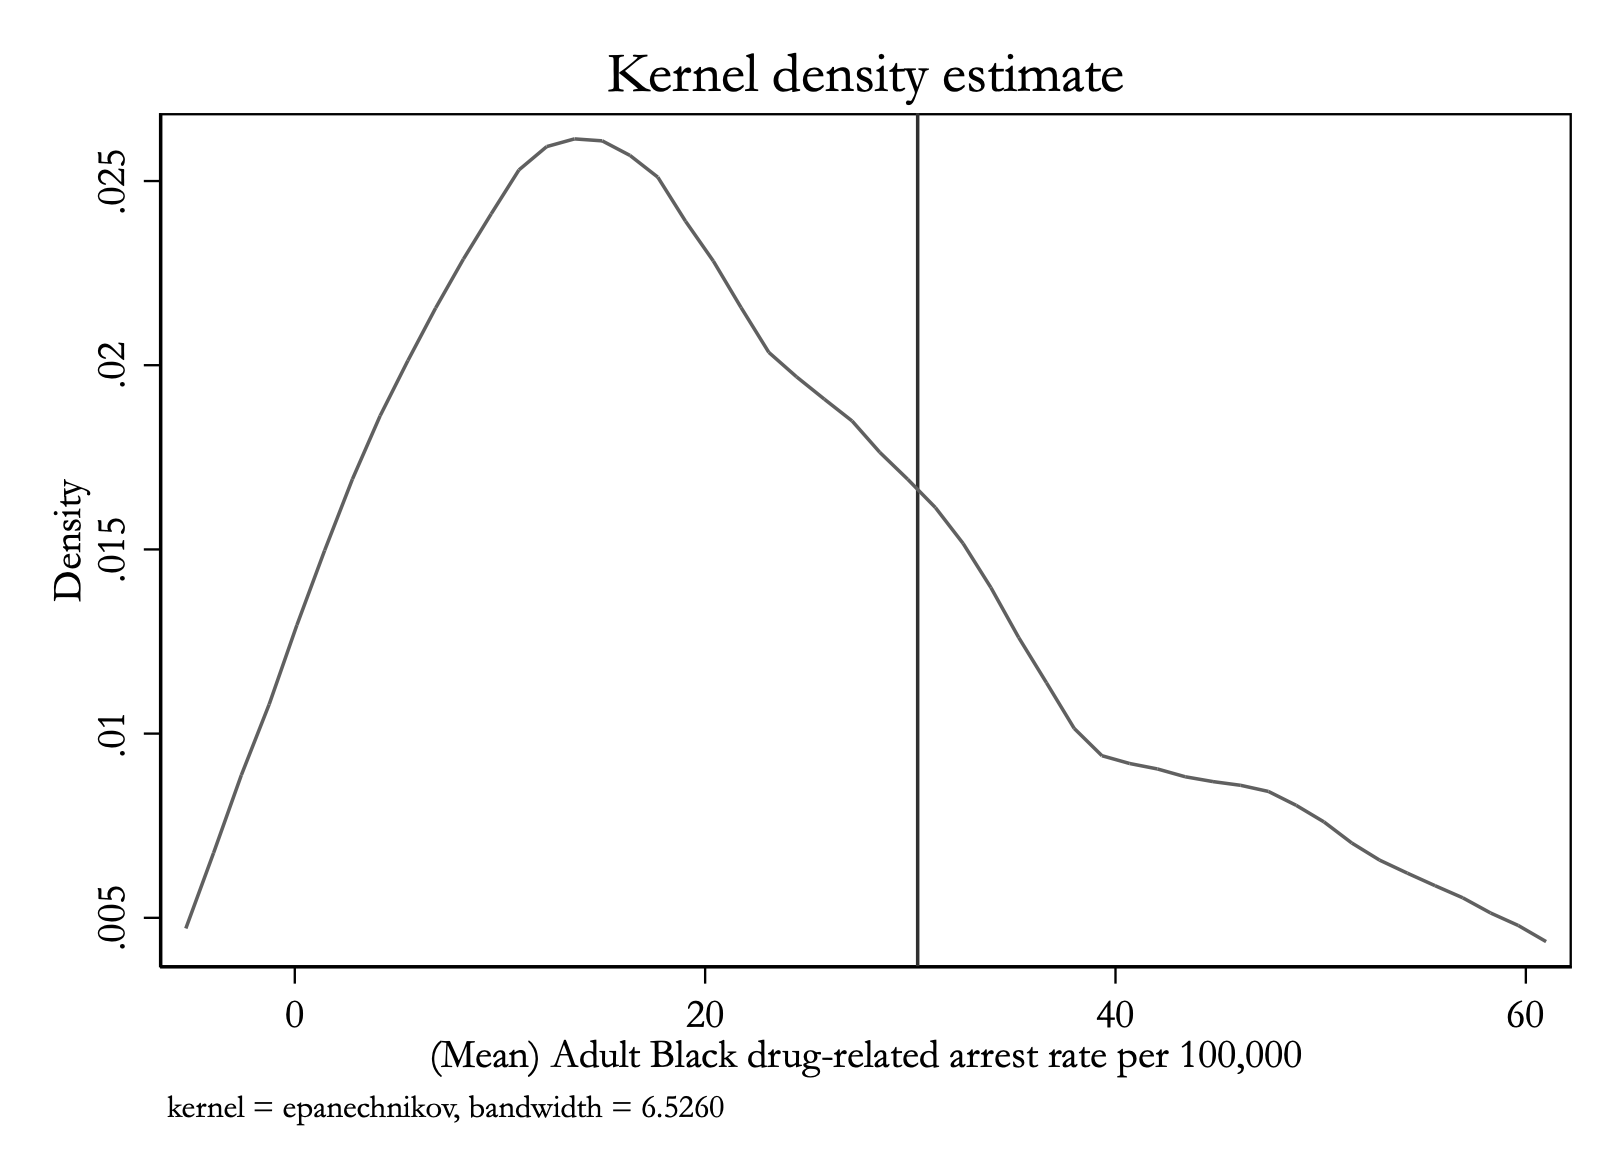
\includegraphics[width=7cm]{descriptive/norm_jb_100000_density_2010.png} }}%
    \label{fig:density_jb}%
  \end{figure}
  \begin{footnotesize}
    \noindent Note: These figures report the kernel density estimates for the normalized drug-related black juvenile arrest rate at the state-by-year level. 
  \end{footnotesize}

